\documentclass[12pt,a4paper]{article}

% Packages
\usepackage[utf8]{inputenc}
\usepackage[margin=1in]{geometry}
\usepackage{graphicx}
\usepackage{amsmath}
\usepackage{amssymb}
\usepackage{hyperref}
\usepackage{cite}
\usepackage{booktabs}
\usepackage{caption}
\usepackage{subcaption}
\usepackage{algorithm}
\usepackage{algorithmic}
\usepackage{xcolor}
\usepackage{float}

% Graphics paths
\graphicspath{
    {open-data/results/presentation/}
    {open-data/results/}
    {open-data/visualizations/zone_analysis/fa_wsl_2018-19/GRID/}
    {open-data/visualizations/zone_analysis/fa_wsl_2018-19/KDE/}
    {open-data/visualizations/zone_analysis/fa_wsl_2020-21/GRID/}
    {open-data/visualizations/possession_patterning_analysis/}
}

% Hyperlink setup
\hypersetup{
    colorlinks=true,
    linkcolor=blue,
    citecolor=blue,
    urlcolor=blue
}

% Title information
\title{\textbf{Using Possession Value to Evaluate Zone Utilization and Spatial Routing in Women’s Football}}

\author{
    Braeden Falzarano \\
    Applied Data Science Capstone \\
    \texttt{[bfalzarano@wesleyan.edu]}
}

\date{\today}

\begin{document}

\maketitle

\begin{abstract}
This paper develops an open-source Possession Value Added (PVA) model for women’s football and applies it to study whether teams’ spatial decisions (i.e., where they play on the pitch and how they route possessions) explain differences in value generation. Using StatsBomb open event data from two seasons of the FA Women’s Super League (2018--19 and 2020--21; 23 team-seasons, approximately 250,000 on-ball actions), we estimate an Expected Threat (xT) surface via a Markov-chain framework on a $6 \times 3$ zone grid and then value each action as the change in xT, with bonuses for progressive passes and carries, line-breaking actions, penalty-box entries, shot assists, carries under pressure, and dribbles. Across 23 team-seasons, PVA per game correlates with goal difference per game at $r_s = .92$, comparable to established metrics such as xG and xT. We then introduce two metrics that measure how much value teams gain or lose from their spatial decisions alone. \textit{Zone Value Added} (ZVA) holds per-zone value constant at the league average and asks how much value a team’s zone distribution adds or subtracts. It explains up to 27\% of a team’s mean PVA, but is heavily confounded by team quality. Removing ZVA from PVA drops Arsenal from 1st to last in league PVA, an implausible shift that suggests ZVA is largely a proxy for zone accessibility rather than a real tactical signal. \textit{Routing Value Added} (RVA) applies the same logic to clustered possession patterns, stratified by starting third, and produces more interpretable shifts in PVA. Middle-of-the-table teams shift up to four positions while the top three remain stable, suggesting that RVA better captures genuine tactical variation in how teams route possessions. The analysis is implemented as a fully documented, open-source framework to allow reproducibility and extension by other researchers.
\end{abstract}

\newpage
\tableofcontents
\newpage

% ============================================================================
\section{Introduction}
% ============================================================================

In the last two decades, football analytics has advanced rapidly from descriptive statistics to advanced models that quantify how actions and locations contribute to scoring opportunities, with metrics like Expected Goals (xG) and Expected Threat (xT) now the standard for assessing on-ball actions. Despite this development, many applications estimate \emph{where} value exists on the pitch, rather than asking how much of a team's value generation is explained by where they choose to play.

This paper studies \textit{spatial allocation} in professional women's football: whether differences in where teams distribute their actions on the pitch and how they route possessions explain differences in the value they generate. We approach this at two levels: (1) \textbf{Zone Level} --- we assign each zone the league-average PVA and measure how much value a team generates strictly through zone allocation by analyzing how often they use each zone relative to league average usage; (2) \textbf{Possession Routing Level} --- we assign each possession pattern the league-average PVA and measure how much value a team generates strictly through possession-patterning by analyzing how often they use each pattern relative to league average usage.

To do this analysis, we developed a \textbf{Possession Value Added (PVA)} model using StatsBomb open event data from two seasons of the FA Women's Super League (2018--19 and 2020--21). Because no pre-computed xT surface exists for the FA WSL, the model estimates one directly from the event data. Following Singh's xT framework \cite{singh_xt_2018}, we model possession as a Markov chain over pitch zones, meaning the expected threat from any zone depends only on which zone the ball is currently in, not on the sequence of zones visited before it arrived there. This memoryless assumption is a deliberate simplification. While possession history does carry information, the current zone captures proximity and angle to goal, which are the most important determinants of future scoring threat. Shot probabilities, zone-to-zone transition probabilities, and expected shot quality (adjusted using StatsBomb's shot-level xG) are estimated from the observed event sequences and used to iteratively compute each zone's expected threat until values stabilize, producing a league- and season-specific pitch-value surface. Each on-ball action is then valued as the change in xT between its start and end zone, with bonuses given for progressive actions, line-breaking plays, penalty-box entries, shot assists, carries under pressure, and dribbles. We then define two complementary metrics, namely \textbf{Zone Value Added (ZVA)} and \textbf{Routing Value Added (RVA)}, that measure how much value a team gains or loses from its spatial decisions, holding per-zone value at the league average.

\paragraph{Contributions.}
This paper contributes an open-source PVA model for women's football, validated against established metrics across two FA WSL seasons. It also introduces two value-added metrics, ZVA at the zone level and RVA at the possession-routing level, that measure how much value teams gain or lose from their spatial decisions.

\section{Related Work}

\subsection{Expected Threat}
Expected Threat (xT) assigns each pitch zone the probability that the current possession results in a goal, given the ball is in that zone \cite{singh_xt_2018}. The model combines (i) the probability of shooting from that zone, (ii) the goal-conversion rate of shots from that zone, and (iii) the probability of moving the ball to another zone and the xT of that destination zone. The pitch is divided into a grid of zones, and all probabilities are estimated from historical event data. xT values are then computed iteratively until they stabilize, yielding a pitch-value surface that increases toward the goal.

\subsection{Possession Value Models}
Possession value models generalize xT by valuing actions according to how they change the expected outcomes of a possession. \textbf{Expected Possession Value (EPV)} models can incorporate tracking data and off-ball context, but require each player’s locations at a given time. This type of tracking data is not available in the StatsBomb open datasets used here \cite{fernandez2019wide}. \textbf{Valuing Actions by Estimating Probabilities (VAEP)} assigns value to actions by modeling changes in the probabilities of scoring and conceding over a short horizon, using supervised learning methods such as gradient-boosted trees \cite{decroos2019vaep}. A metric such as \textbf{On Ball Value (OBV)} is comparable to the PVA metric developed here, but StatsBomb’s proprietary modeling choices and paid access motivate the development of an open-source model that promotes research and allows reproducibility \cite{statsbomb_obv}. It should be noted that the zone-level and possession-routing analyses in this paper could be conducted with action-level values from VAEP or any comparable model. We chose to develop our own PVA model for several reasons. First, we wanted an interpretable framework. By modeling each action as an xT change plus explicit bonuses, the value of any action can be traced directly to how it contributed to moving the ball through space and to contextual features without relying on a learned "black-box" model. Second, building the model from scratch on StatsBomb open data ensures that any researcher can replicate the pipeline without access to proprietary tools or pre-trained models. This not only allows the framework in the current study to be easily applied to other competitions and seasons within the StatsBomb open-data repository, but also supports future extensions and changes by the research community if they see fit.

\subsection{Spatial Utilization and Tactical Analysis}
Prior work has examined spatial structure and control in football, as well as zone-based summaries (i.e., usage maps and transition patterns) used to characterize team style \cite{amichay2025spatial, gu2024spacecontrol}. However, fewer studies evaluate how much of the variation in team value is explained by spatial distribution alone, which this paper aims to do.

\subsection{Possession Sequence Analysis}
Several studies have applied clustering and possession-pattern clustering methods to identify recurring tactical patterns. Decroos et al.\ \cite{decroos2018automatic} cluster phases of play using dynamic time warping on event sequences and then apply sequential pattern mining to identify recurring tactics. Our work takes a different approach. We represent each possession as a continuous spatial trajectory, cluster within each starting third using $k$-medoids, and use the resulting pattern frequencies to define a Routing Value Added metric (RVA).


% ============================================================================
\section{Research Problem}
% ============================================================================

\subsection{Problem Statement}
This paper examines \emph{spatial allocation} in professional women’s football. We ask how much of the variation in teams’ value generation is explained by where they distribute their actions on the pitch and which possession routes they follow. Using the PVA model framework, we hold per-zone (or per-pattern) value constant at the league average and measure how much value each team gains or loses purely from its distribution of actions across zones or possession patterns. This approach is of interest because it isolates where and how teams choose to play, rather than just how much raw talent they possess.

\subsection{Research Questions}

\textbf{RQ1 (Model validity):} Does the PVA model built from open event data produce action-level values that correlate with team performance outcomes comparably to established metrics such as xG and xT?

\textbf{RQ2 (Zone usage footprints):} Do FA WSL teams use pitch zones at significantly different rates from one another?

\textbf{RQ3 (Zone allocation):} How much of a team’s overall PVA is explained by its distribution of actions across zones (ZVA), holding per-zone value at the league average?

\textbf{RQ4 (Possession routing):} Do teams’ possession-routing patterns differ in value, and does Routing Value Added (RVA) capture tactical information beyond what ZVA captures?

% ============================================================================
\section{Methodology}
% ============================================================================

\subsection{Overview}
The methodology has three stages: (i) construct and validate the PVA model from event data; (ii) measure how much value each team gains or loses from its zone usage (ZVA), holding per-zone value at the league average; (iii) cluster possession sequences and compute Routing Value Added (RVA) to capture spatial-routing context beyond the zone grid.

\subsection{xT Model Construction}
Because publicly available xT values do not exist for the FA WSL, we estimate our own xT surface from the event data within each league-season. We model a possession as a sequence of transitions over discrete pitch zones. Let $z \in \{1,\dots,18\}$ index the zones of the pitch. From each zone, the possession can (i) end in a shot, (ii) transition to another zone via a ball-moving action, or (iii) end via loss of possession.

For each zone $z$, xT is defined as the probability that the current possession results in a goal, given the ball is in $z$:
\begin{equation}
xT(z)
=
\underbrace{
P(\text{shot}\mid z)\cdot \overline{xG}_z
}_{\text{Immediate shooting value}}
\;+\;
\underbrace{
P(\text{move}\mid z)\cdot \sum_{z'=1}^{18} P(z' \mid \text{move}, z)\cdot xT(z')
}_{\text{Continuation value from moving the ball}}
\end{equation}

where $\overline{xG}_z$ is the average xG of shots taken from zone $z$, and the summation is over all 18 possible destination zones that the ball could move to from the current zone. All probabilities are estimated from the observed actions within each league-season. Here, \emph{move} is a ball-moving action that continues the possession (i.e., a completed pass or carry). We compute $P(\text{shot}\mid z)$ from the observed shot frequency in each zone. For $\overline{xG}_z$, we use the average of StatsBomb's shot-level xG estimates for shots taken in zone $z$, rather than raw goal-conversion rates, which provides a sufficient estimate of shot quality given the limited sample of shots in some areas of the pitch. We estimate transition probabilities $P(z'\mid \text{move}, z)$ from completed ball-moving actions that start in $z$. We compute xT by iteratively updating these values until they stabilize, producing a pitch-value surface that can be visualized and used for downstream analysis.

\paragraph{Pitch Grid Discretization.}
The pitch is divided into a $6 \times 3$ grid of 18 zones (six columns spanning sideline to sideline, three rows spanning endline to endline). Each pitch third, namely defensive, midfield, and attacking, contains two columns and three rows, giving six zones per third. This design is chosen to capture meaningful tactical distinctions between zones. For example, it separates not just left, center, and right midfield, but also whether the ball is in a deeper or more advanced midfield position. At the same time, the grid zones are large enough that every team has at least several hundred actions in each zone, ensuring reliable probability estimates. Figure~\ref{fig:xt_grid} shows the resulting league-average xT surface, illustrating how expected threat increases toward the goal.

\begin{figure}[H]
\centering
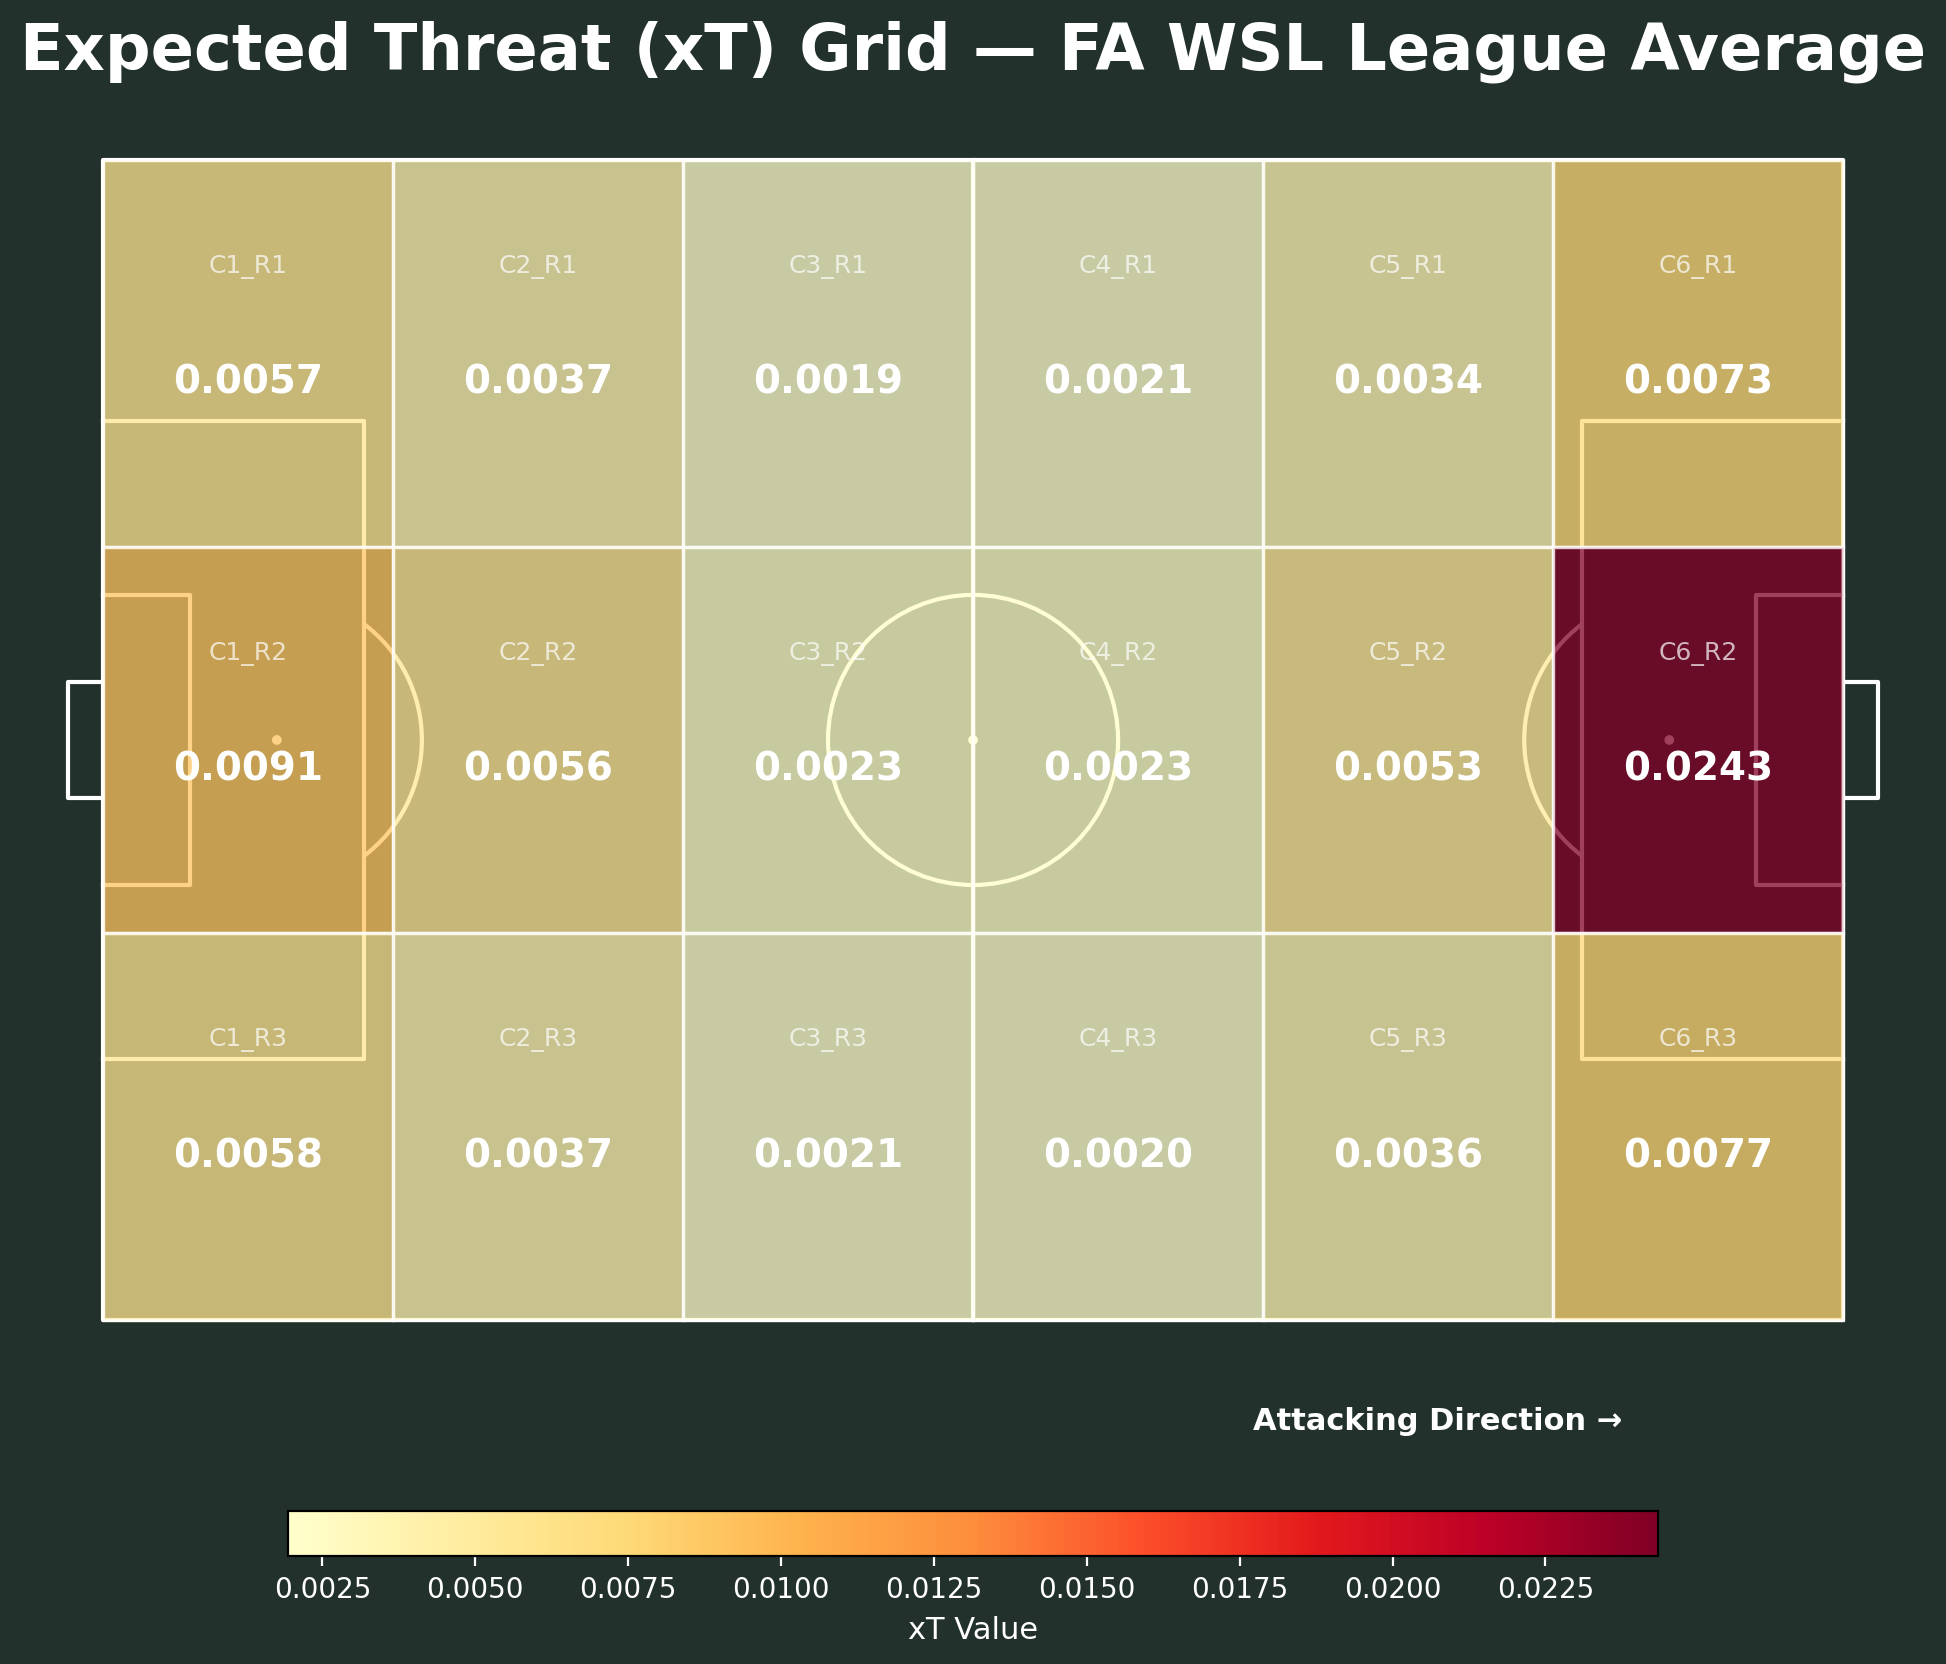
\includegraphics[width=0.85\textwidth]{xt_grid_league_average.png}
\caption{League-average xT surface across the $6 \times 3$ zone grid for the FA WSL. Each cell shows the probability that a possession results in a goal given the ball is in that zone. Values increase toward the attacking end of the pitch, with C6\_R2 (the central zone directly in front of goal) carrying the highest xT.}
\label{fig:xt_grid}
\end{figure}

\subsection{Possession Value Added (PVA) for Actions}
Given an xT surface, the baseline value of an on-ball action $a$ that moves the ball from zone $z$ to zone $z'$ is the change in expected threat:
\begin{equation}
V_{\text{base}}(a) = xT(z') - xT(z).
\end{equation}
PVA builds on this base value by adding bonuses for action characteristics that the xT change alone does not capture.

\paragraph{Bonus adjustments.}
These bonuses include: progressive passes and carries (actions that advance the ball a substantial distance toward goal), line-breaking actions (in the context of this model, defined as actions that cross from one pitch third to the next, e.g., midfield to attacking third), penalty-box entries (passes or carries that end inside the penalty area), shot assists (the pass immediately preceding a shot), carries under pressure (using StatsBomb's pressure indicators), and successful dribbles (1v1 take-ons that beat a defender). These features matter because $V_{\text{base}}$ only captures the value of moving the ball from one zone to another. It cannot distinguish, for example, a progressive pass that advances 15 yards within a zone from a short lateral pass in the same zone, even though the progressive pass is more likely to lead to a goal. To set each bonus weight, we compare actions with and without a given feature that end in the same zone, pooling across all league-seasons. By comparing actions with the same destination zone, we control for the spatial movement already captured by $V_{\text{base}}$, and the remaining difference in goal-scoring outcomes indicates how much additional value the feature itself contributes. The final weights are rounded and then input into the model.

\paragraph{Shots and turnovers.}
For shots, we treat the event xG as the immediate expected value of the attempt and adjust relative to the pre-shot state:
\begin{equation}
V_{\text{shot}} = xG - xT(z_{\text{shot}}).
\end{equation}
For turnovers (failed passes, dispossessions, miscontrols), we assign a negative value reflecting the threat the opponent generates after winning the ball. Rather than using a simple heuristic, we build an empirical turnover consequence model. For each observed turnover in zone $z$, we track the opponent’s subsequent actions (up to 10) until the original team regains possession, summing the xT of each opponent action location. Averaging across all turnovers in each zone gives the empirical turnover consequence $\overline{T}_z$, and the turnover cost is:
\begin{equation}
V_{\text{turnover}}(z) = -\overline{T}_z
\end{equation}
For zones where no turnovers were observed in the data ($N_z = 0$), we fall back to the xT of the mirrored zone (flipping coordinates to the opponent’s attacking direction) as an estimate:
\begin{equation}
\overline{T}_z = xT\bigl(\text{flip}(z)\bigr) \quad \text{when } N_z = 0
\end{equation}

\paragraph{Defensive actions.}
Defensive events that end an opponent’s possession (e.g., interceptions, ball recoveries) use the same empirical turnover consequence model, but in reverse. When a team wins the ball in zone $z$, the defensive value has two components: (i) the threat denied to the opponent, estimated as $\overline{T}_{z'}$ where $z'$ is the mirrored zone from the opponent’s attacking perspective; and (ii) the threat created by regaining possession, estimated as $\overline{T}_z$ at the location the ball is recovered.

\subsection{Model Assessment}\label{sec:calibration}
Because StatsBomb's OBV metric is both proprietary and unavailable to get access to for this project, we assess the model using metrics available through open source data.

\paragraph{Benchmark comparison.}
We benchmark PVA per game against nine established metrics: xG, xT, possession share, progressive passes, progressive carries, line breaks, penalty-box entries, final-third entries, and pressure actions. We do this by computing Spearman correlations with goals per game and goal difference per game at the team-season level. This is done both per league and pooled across all 23 team-seasons.


\subsection{Zone Value Added (ZVA)}

Let $u_{t,z}$ denote the \emph{utilization} of zone $z$ by team $t$ (i.e., the proportion of team $t$’s actions that occur in zone $z$):
\begin{equation}
u_{t,z}
=
\frac{n_{t,z}}{N_t}
\end{equation}
where $n_{t,z}$ is the number of actions taken by team $t$ in zone $z$ and $N_t = \sum_z n_{t,z}$ is the total number of actions by team $t$. We then find the leave-one-out (LOO) league baseline, which becomes the reference level for team $t$. This reference utilization, defined as $\bar{u}_{\text{LOO},z}$, is the mean utilization of the other teams in the league. We use a LOO approach so that a team never influences its own baseline.

\paragraph{Definition.}
ZVA measures how much value a team gains or loses from where it distributes its actions on the pitch. It holds PVA per-zone constant at the league average and asks, given the known value of each zone, how much value does this team’s zone distribution add or subtract compared to the league-average distribution?
\begin{equation}
\text{ZVA}_t = \sum_{z} \bigl(u_{t,z} - \bar{u}_{\text{LOO},z}\bigr) \cdot \bar{v}_z
\end{equation}
where $\bar{v}_z$ is the league-average PVA per action in zone $z$ and $\bar{u}_{\text{LOO},z}$ is the LOO league-average utilization of zone $z$. The team’s own per-zone PVA does not enter the equation. This is done intentionally to attempt to isolate the contribution of \emph{where} a team plays, from \emph{how well} it plays there. A team earns positive ZVA by over-utilizing zones with positive league-average PVA or under-utilizing zones with negative league-average PVA, relative to the LOO baseline. Conversely, a team earns negative ZVA by under-utilizing positive-PVA zones or over-utilizing negative-PVA zones. In practice, this means that teams that more frequently utilize high-value zones of the pitch will tend to have a higher ZVA. ZVA can be expressed both as a raw number and as a percentage of the team’s overall mean PVA. The latter helps contextualize its magnitude of contribution to the team’s overall performance.

\paragraph{Statistical testing.}
We apply three different tests. First, we use chi-square goodness-of-fit tests to assess whether each team’s zone usage distribution differs significantly from the league average, and then use pairwise chi-square tests of homogeneity to test whether every pair of teams uses zones at different rates. Last, we use one-sample $t$-tests to test whether each team’s mean PVA in a given zone differs from the LOO league mean for that zone, identifying zones of significant over or under performance. Because we run a separate test for every team/zone combination, a standard $\alpha = 0.05$ threshold would produce ~8 significant results out of 162 total tests, just by random chance. If we were to find 7 other "actual" significant results, we would then have a 53\% false positive rate. To address this, we apply a false discovery rate (FDR) correction, which ensures that at most 5\% of the \emph{discoveries themselves} are expected to be false.

\subsection{Possession Patterning and Routing Value Added}
While zones summarize individual actions at fixed locations, possession patterning captures the spatial \emph{shape} of full possession sequences (i.e., the routes teams take across the pitch).

\paragraph{Possession extraction and representation.}
We extract every multi-action possession from the event data and represent each as a spatial trajectory: the ordered sequence of $(x, y)$ coordinates visited during the possession. Each trajectory is resampled to a fixed-length vector of 20 equally spaced waypoints via linear interpolation, producing a standardized representation regardless of the number of original actions.

\paragraph{Stratified clustering.}
Possessions are stratified by their starting third (defensive, midfield, or attacking) before clustering, so that clusters capture real routing patterns in each phase of play. Before stratification was implemented, the clustering was simply separating possessions by distance traveled, rather than capturing pattern nuance. Within each stratum, we apply $k$-medoids clustering (FasterPAM algorithm) using Euclidean distance on 20-waypoint vectors. Because standard metrics like silhouette score tend to favor very low values of $k$ (e.g., 2 or 3), which fail to capture the actual diversity of possession routes in a soccer match, selecting the number of clusters $k$ requires an alternative, context-based method. To ground the choice of $k$, we first perform \emph{route scouting}: each possession is mapped to a coarse grid-route fingerprint, defined as the sequence of cells visited on any given possession on a $3 \times 3$ grid (e.g., ``DL-MC-AR''). We count how many distinct routes appear at several frequency thresholds. Route scouting revealed that each stratum contains dozens of distinct routes with meaningful sample sizes, confirming that low values of $k$ found by silhouette scores were collapsing different possession patterns into the same clusters. At the same time, using every observed route found by the route-scouting approach made clusters too small for reliable team-by-team analysis and too difficult to interpret visually. We therefore selected $k$ to balance the route-scouting pattern diversity with analytical and visual interpretability. We landed on 18 clusters each for the defensive and midfield strata, and 9 for the attacking stratum. At these values of $k$, route scouting confirmed that each cluster corresponds to a possession route appearing in roughly 0.5--1\% or more of possessions. Silhouette scores, Calinski--Harabasz scores, and total distance (elbow) were evaluated at these values as a secondary check, and the resulting clusters were visually inspected to verify that each pattern represents a distinguishable possession route. Possessions whose distance to the nearest medoid exceeds the 75th percentile are marked as unassigned to improve cluster coherence.

Let $f_{t,c}$ denote the fraction of team $t$’s possessions assigned to cluster $c$:
\begin{equation}
f_{t,c} = \frac{p_{t,c}}{P_t}
\end{equation}
where $p_{t,c}$ is the number of team $t$’s possessions in cluster $c$ and $P_t = \sum_c p_{t,c}$ is the total number of assigned possessions for team $t$. As with ZVA, we compute a LOO league baseline $\bar{f}_{\text{LOO},c}$ so that a team never influences its own reference level.

\paragraph{Definition.}
RVA measures how much value a team gains or loses from which possession patterns it favors. It holds per-pattern PVA constant at the league average and asks, given the known value of each pattern, how much value does this team’s pattern distribution add or subtract compared to the league-average distribution?
\begin{equation}
\text{RVA}_t = \sum_{c} \bigl(f_{t,c} - \bar{f}_{\text{LOO},c}\bigr) \cdot \bar{v}_c
\end{equation}
where $\bar{v}_c$ is the LOO league-average mean PVA per possession in cluster $c$ and $\bar{f}_{\text{LOO},c}$ is the LOO league-average frequency of cluster $c$. The interpretation mirrors ZVA, as a team earns positive RVA by over-utilizing high-value possession patterns or under-utilizing low-value ones, and negative RVA from the reverse. In practice, teams that more frequently use possession routes that generate high PVA will tend to have a higher RVA. RVA is computed within each stratum and summed to produce a team-level total.

% ============================================================================
\section{Data and Implementation}
% ============================================================================

\subsection{Data Source and Sample}
We use StatsBomb’s open event dataset for two seasons of the FA Women’s Super League (2018--19 (11 teams) and 2020--21 (12 teams)), totaling 23 team-seasons and approximately 250,000 on-ball actions. The data are distributed as JSON files through the StatsBomb open-data repository on GitHub \cite{statsbomb_open_data}. Events are recorded using StatsBomb’s standardized pitch coordinate system ($120 \times 80$ arbitrary units) and include 10 on-ball action types: passes, carries, shots, ball recoveries, blocks, dribbles, dribbled past, dispossessions, interceptions, and miscontrols. Shot events have an expected goals (xG) estimate from StatsBomb, which we use as the immediate expected value for shot attempts. For possession patterning, we additionally include actions from the FA WSL 2019--20 season and the NWSL 2018 season (both incomplete seasons of data) to increase the volume of actions and thus increase the number of possession sequences available to use for clustering. These additional seasons contribute only to fitting the cluster centroids and not for the RVA computations and analysis, which use only the 23 FA WSL 2018--19 and 2020--21 team-seasons.

\subsection{Preprocessing}
We apply the following preprocessing steps to each league-season:
\begin{enumerate}
    \item Load all match event files for the season.
    \item Retain events with valid locations and (where applicable) end locations.
    \item Normalize direction of play by flipping coordinates so all possessions are represented as attacking in a consistent direction.
    \item Assign each action to a zone on the $6 \times 3$ grid using its start location.
\end{enumerate}
For zone-level visualizations, we exclude the ``danger zone'' (column 6, row 2: the central area directly in front of goal) because PVA values in this zone are dominated by shots and are extreme relative to all other zones, which would distort visual comparisons. The danger zone is retained in all statistical tests and ZVA computations.

\subsection{Implementation and Reproducibility}
All data preprocessing, modeling, and visualization steps are implemented in Python. The PVA model is implemented in a way that allows it to be applied to any StatsBomb competition and season. The full codebase, including parameter settings, grid definitions, and analysis scripts, is available as an open-source repository on GitHub.

% ============================================================================
\section{Results}
% ============================================================================

\subsection{PVA Model Validation (RQ1)}

We first assess whether PVA captures meaningful variation in team quality by doing a benchmark analysis against nine established metrics. Table~\ref{tab:benchmark} reports Spearman correlations between each metric (per game) and two season outcomes (goals per game and goal difference per game) pooled across all 23 team-seasons.

\begin{table}[H]
\centering
\caption{Spearman correlations between attacking metrics and season outcomes, pooled across 23 team-seasons (FA WSL 2018--19 and 2020--21). All correlations significant at $p < .001$.}
\label{tab:benchmark}
\begin{tabular}{lcc}
\toprule
\textbf{Metric (per game)} & \textbf{Goals/Game} & \textbf{GD/Game} \\
\midrule
PVA             & .927 & .916 \\
xT              & .937 & .917 \\
xG              & .933 & .913 \\
Possession \%   & .916 & .925 \\
Final 3rd Entries & .933 & .935 \\
Prog.\ Passes   & .928 & .929 \\
Pen Box Entries  & .921 & .911 \\
Line Breaks      & .910 & .912 \\
Prog.\ Carries   & .856 & .877 \\
Pressure Actions & .664 & .663 \\
\bottomrule
\end{tabular}
\end{table}

PVA per game correlates with goal difference at $r_s = .916$ and with goals per game at $r_s = .927$, placing it in the same range as xG ($r_s = .913$) and xT ($r_s = .917$). These relationships hold within each season individually: $r_s = .907$ (GD/Game, 2018--19, $n = 11$) and $r_s = .965$ (GD/Game, 2020--21, $n = 12$).

Figure~\ref{fig:benchmark} visualizes these correlations as a dot plot, confirming that PVA performs comparably to the individual metrics it is constructed from.

\begin{figure}[H]
\centering
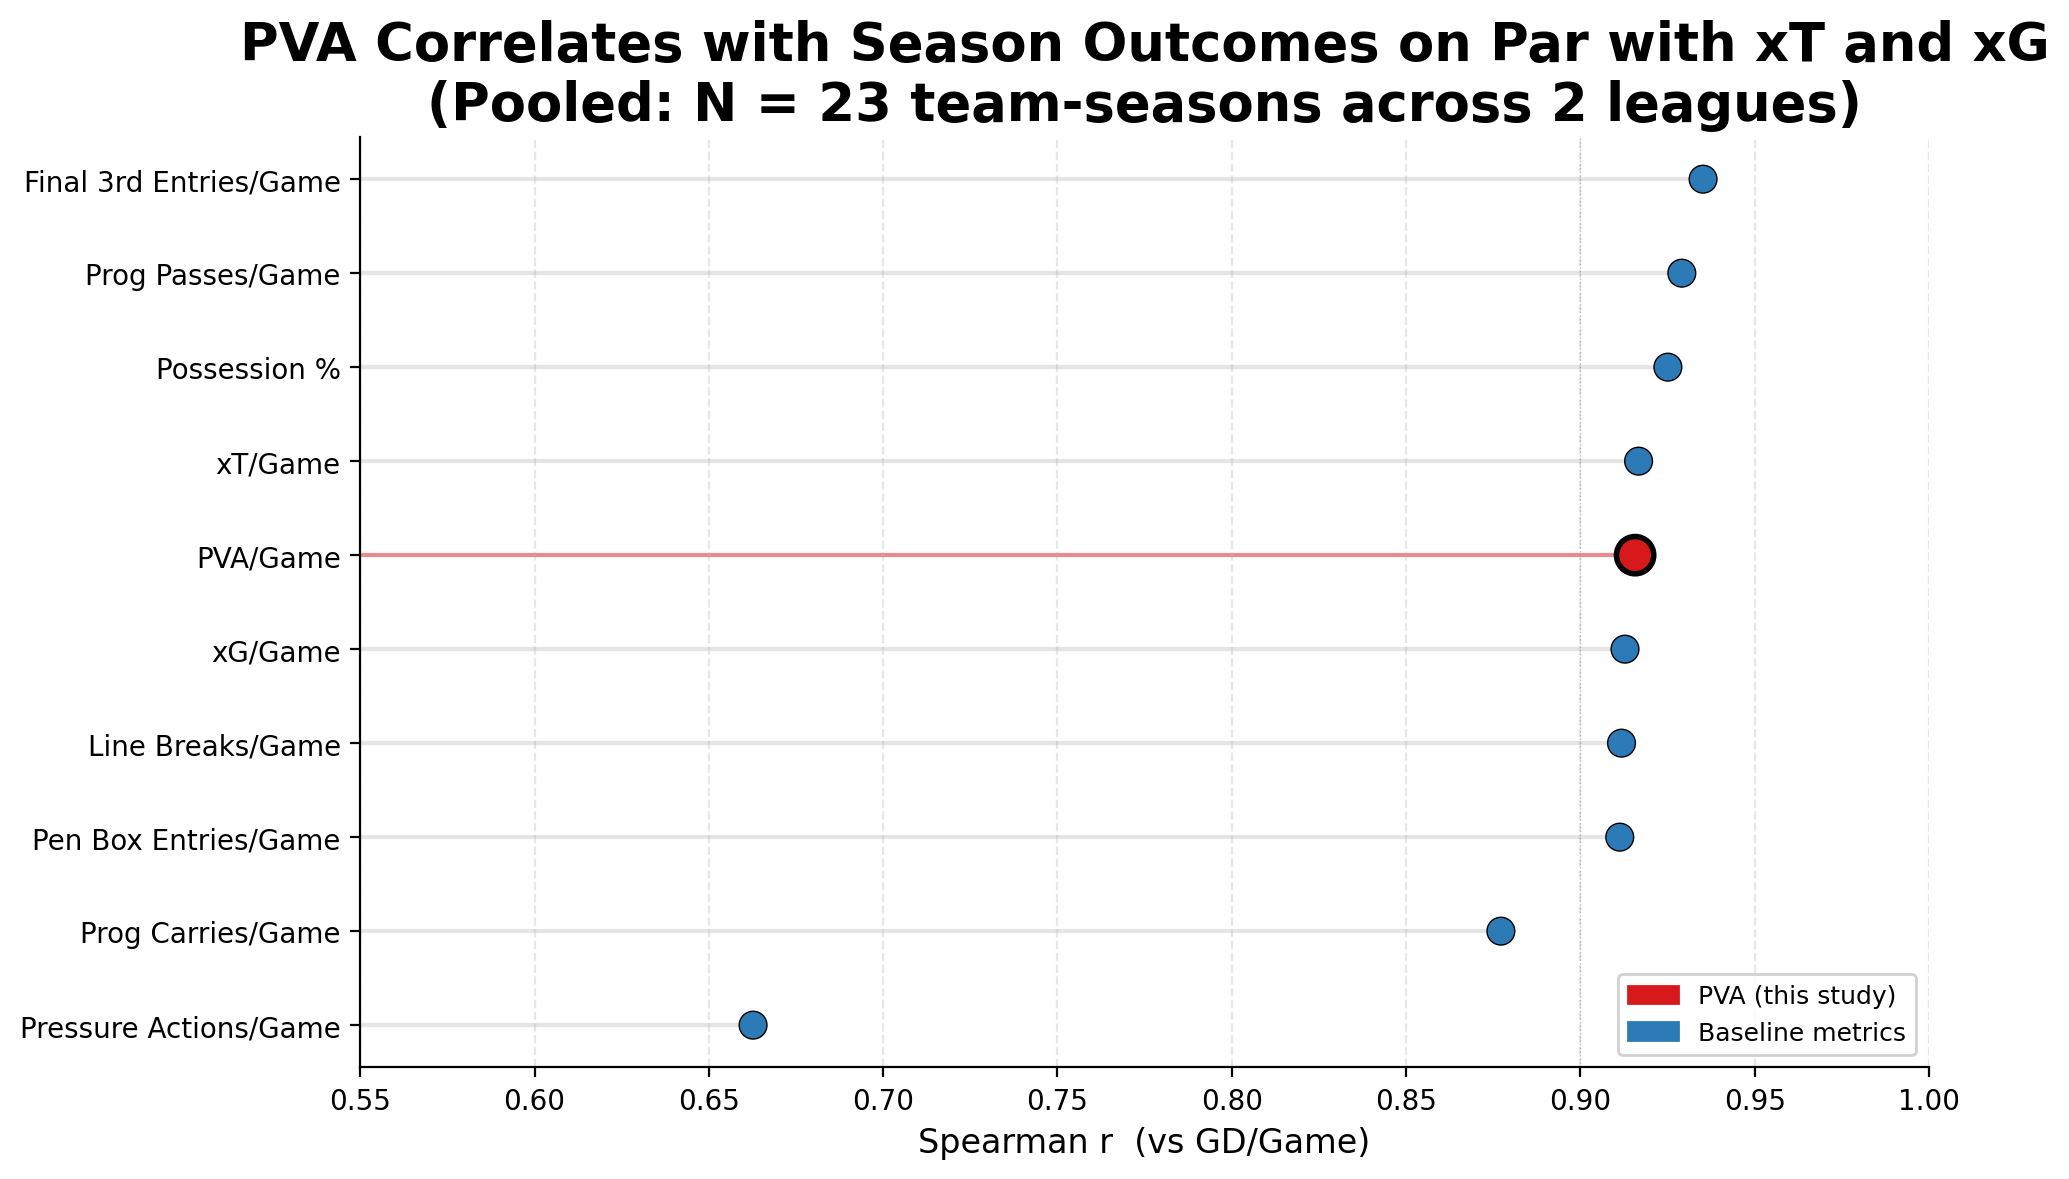
\includegraphics[width=0.85\textwidth]{metric_benchmark_dotplot.png}
\caption{Spearman rank correlations between various metrics (per game) and season outcomes across 23 team-seasons. PVA (highlighted) performs comparably to xG and xT.}
\label{fig:benchmark}
\end{figure}

The above results address RQ1: the PVA model produces team-level value that correlates with performance outcomes at least as well as established metrics.

% --------------------------------------------------------------------------
\subsection{Zone Analysis}

\subsubsection{Zone Usage Distinctiveness (RQ2)}\label{sec:rq2}

We next test whether FA WSL teams use pitch zones at significantly different rates from one another.

\paragraph{Team vs.\ league.}
Chi-square goodness-of-fit tests comparing each team's zone usage distribution against the league average are significant for all 23 team-seasons ($\chi^2(17)$ ranging from 96.5 to 1{,}543.6, $p < .001$ in every case). The wide range of $\chi^2$ values reflects substantial variation in how much teams deviate from the league spatial profile: Arsenal (2018--19, $\chi^2 = 1{,}543.6$) has the most distinctive zone distribution, while West Ham (2020--21, $\chi^2 = 96.5$) is closest to the league average.

\paragraph{Pairwise Team vs.\ Team.}
Pairwise chi-square tests of homogeneity confirm that every pair of teams has a statistically unique zone usage distribution. In 2018--19, all 55 of 55 pairs ($\binom{11}{2}$) are significant at $p < .001$. In 2020--21, 65 of 66 pairs ($\binom{12}{2}$) are significant at $p < .001$, with the remaining pair (Everton vs.\ Tottenham, $\chi^2 = 36.75$, $p = .004$) significant at $p < .01$. $\chi^2$ statistics range from 36.75 to 1,145.4 across 121 total pairwise comparisons.

Figures~\ref{fig:usage_facet} and~\ref{fig:usage_facet_kde} display each team's zone usage in 2018--19, illustrating the variety of spatial footprints across the league. Figure~\ref{fig:usage_facet} uses the same $6 \times 3$ zone grid as the rest of the analysis, so each cell corresponds directly to the zones used in the chi-square tests and ZVA calculations. Figure~\ref{fig:usage_facet_kde} presents the same data using kernel density estimation (KDE), which smooths values across continuous space rather than binning them into fixed zones. The KDE view reveals finer spatial patterns that the grid cannot capture. Used together, the two representations offer both a discrete and continuous spatial perspective on the same underlying data.

\begin{figure}[H]
\centering
\begin{subfigure}[b]{\textwidth}
    \centering
    
\includegraphics[width=\textwidth]{team_comparison_by_category/03_all_teams_usage_density.png}
    \caption{$6 \times 3$ grid. Darker zones indicate higher proportions of a team's actions.}
    \label{fig:usage_facet}
\end{subfigure}

\vspace{0.5em}

\begin{subfigure}[b]{\textwidth}
    \centering
    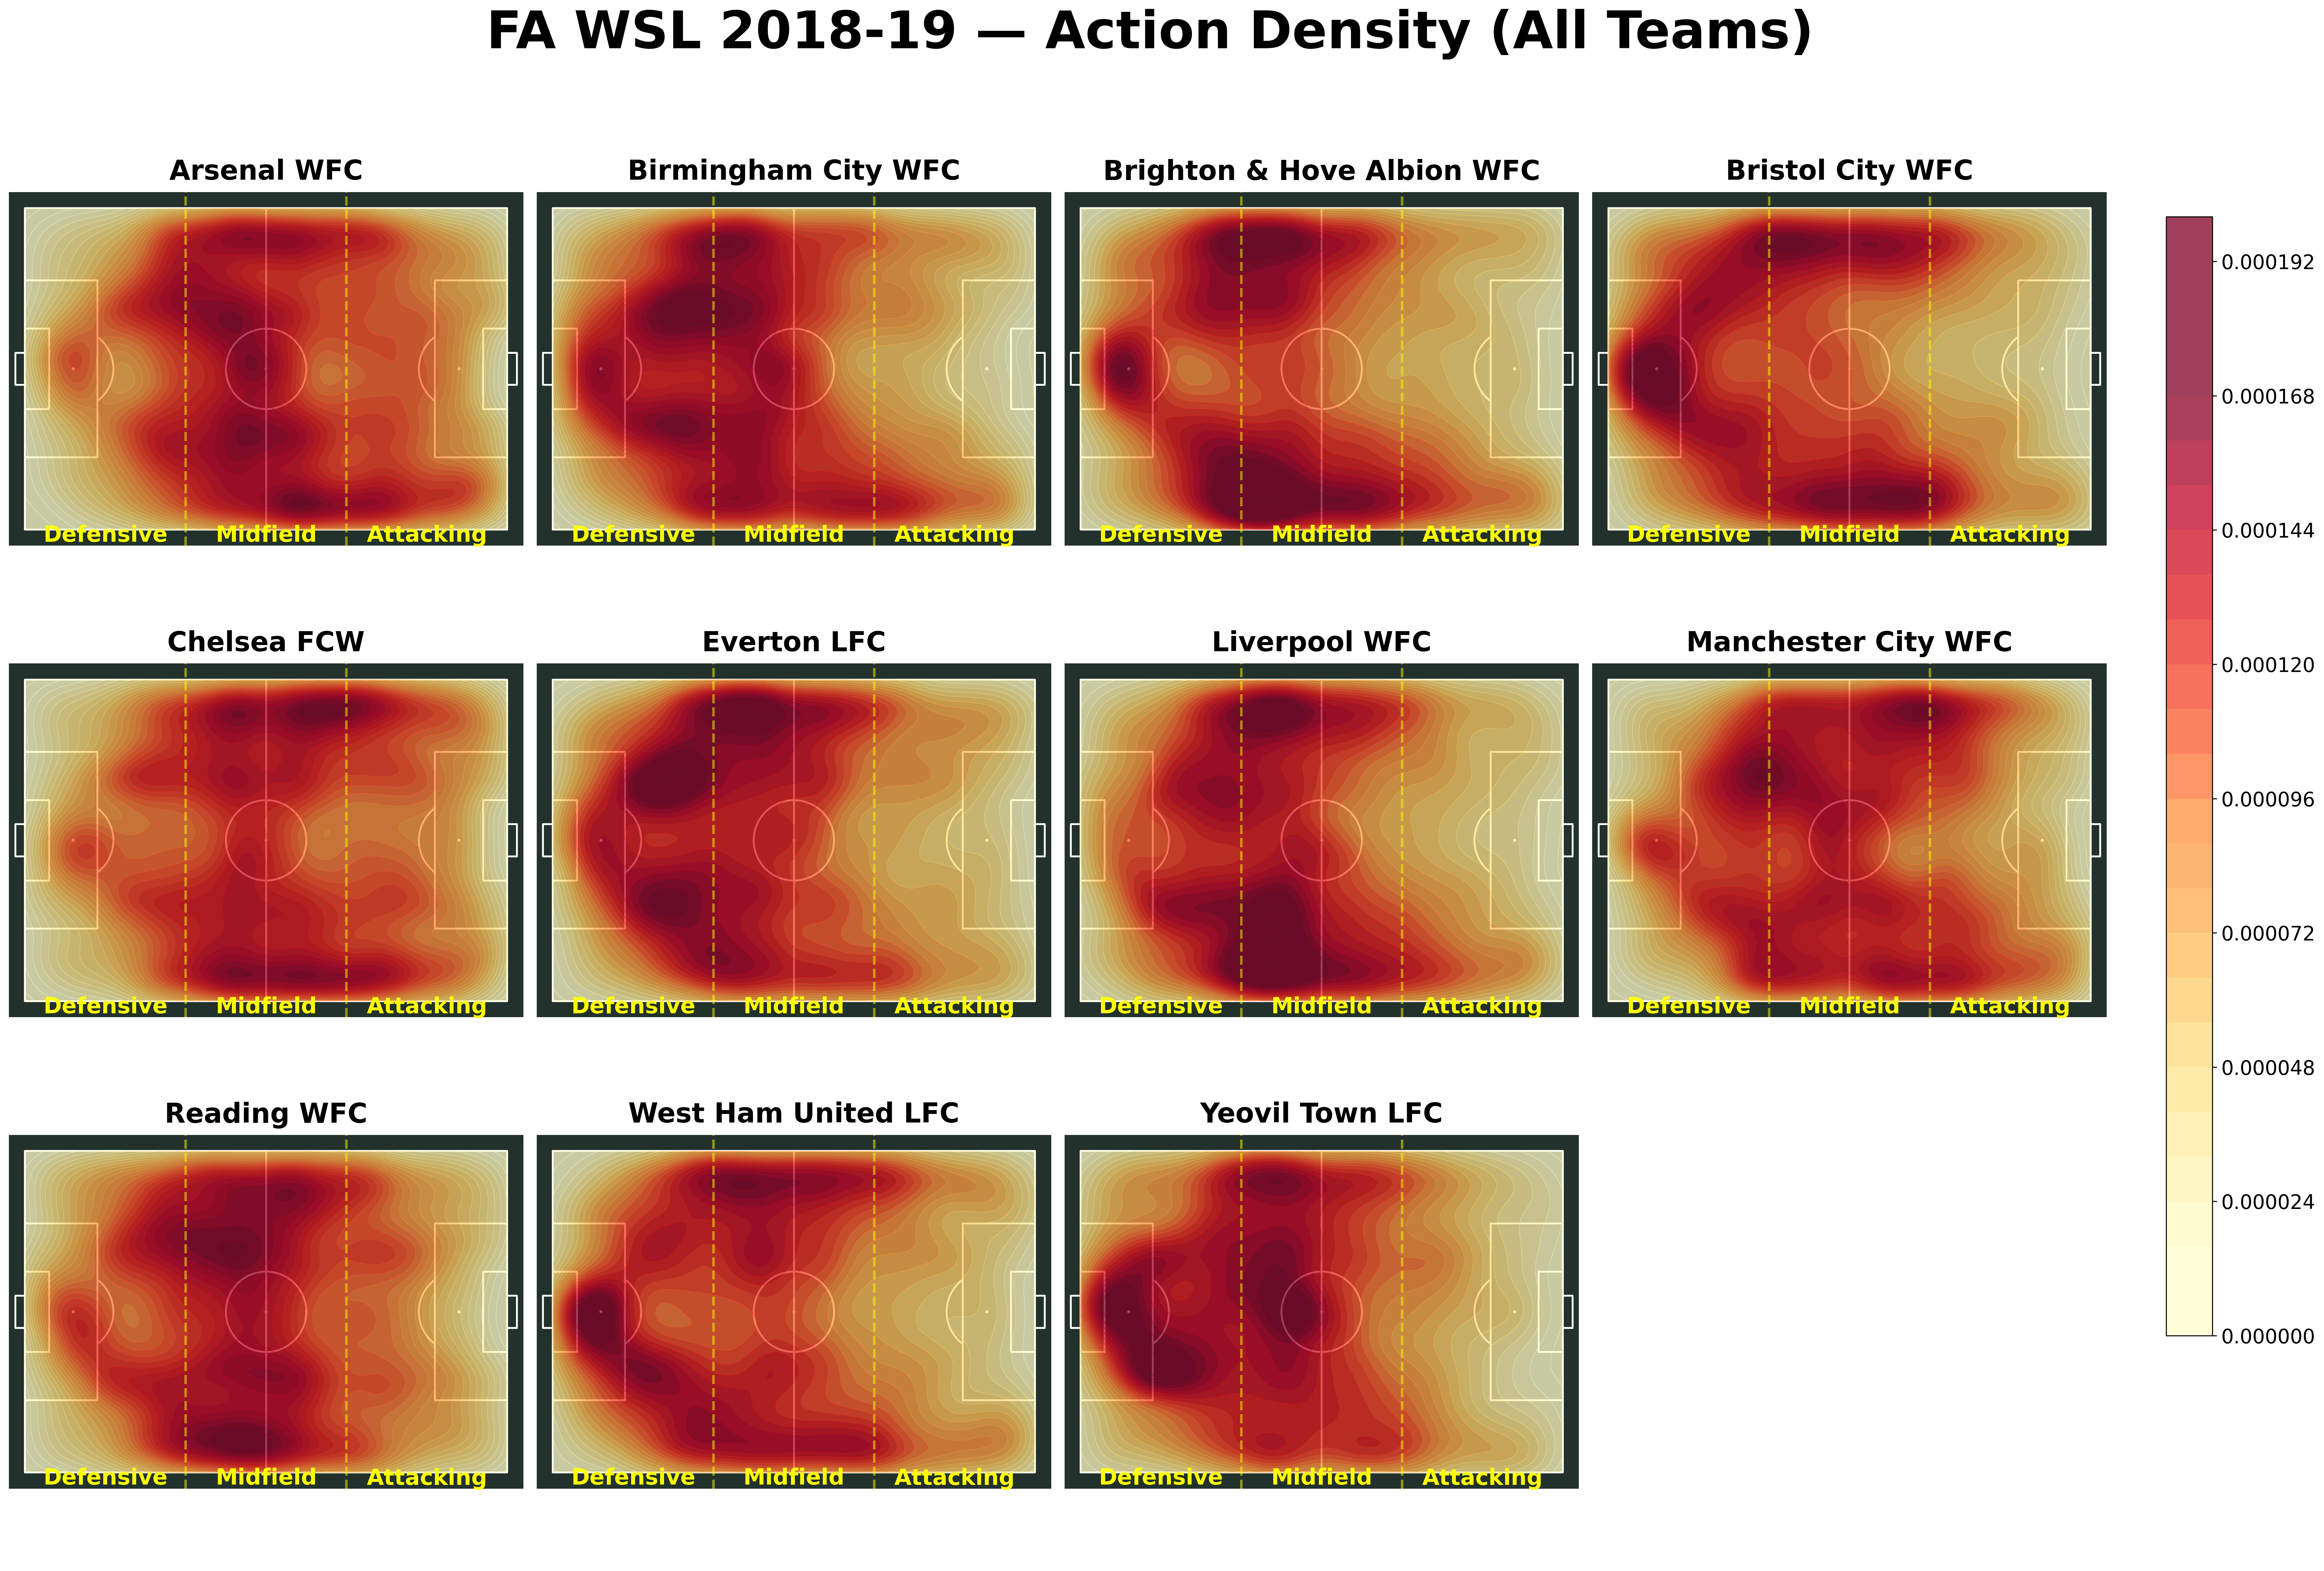
\includegraphics[width=\textwidth]{open-data/visualizations/zone_analysis/fa_wsl_2018-19/KDE/team_comparison_by_category/03_all_teams_usage_density.png}
    \caption{KDE. The same data smoothed across continuous space using kernel density estimation.}
    \label{fig:usage_facet_kde}
\end{subfigure}
\caption{Zone usage density for each team in the FA WSL 2018--19 season. Each team's spatial footprint is statistically unique compared to every other team. Note that the color scales differ between the two representations due to differences in how grid cells and KDE surfaces distribute density.}
\label{fig:usage_both}
\end{figure}

These results address RQ2: every team in both seasons has a unique statistically significant zone usage footprint.

% --------------------------------------------------------------------------
\subsubsection{Zone-Level Performance Differences}

Using one-sample $t$-tests (FDR-corrected) comparing each team's mean PVA in a given zone against the LOO league mean, we find a total of 18 significant team-zone combinations in 2018--19 and 17 in 2020--21 (at $q < .05$). Two zones dominate the significant results: C1\_R2 (center of the defensive third) and C2\_R2 (center of the deep midfield). In 2018--19, 7 of 11 teams show significant deviations in C1\_R2, and 5 of 11 in C2\_R2. Looking into the team-by-team results, we see that the top teams (Arsenal, Chelsea, Manchester City) often perform \emph{below} the league average in these deep central zones, while weaker teams (Yeovil Town, Liverpool, Bristol City) perform \emph{above} the league mean there. This likely reflects the fact that stronger teams tend to spend proportionally more of their time in attacking zones, meaning actions in deep areas are disproportionately low-value clearances and recycling passes, while weaker teams generate a larger share of their value from defensive recoveries and creating turnovers in these zones.

Figures~\ref{fig:buildup_grid} and~\ref{fig:buildup_kde} (shown on the next page) visualize these team-vs-league deviations across the full pitch in both grid and KDE form. Both figures show how each team's mean "buildup PVA" compares to the league average. Buildup PVA includes all actions except those in the danger zone (Zone C6\_R2). Warm colors (red/orange) indicate zones where the team generates more value per action than the league mean, and cool colors (blue) indicate zones where it generates less.

\begin{figure}[H]
\centering
\begin{subfigure}[b]{\textwidth}
    \centering
    
\includegraphics[width=\textwidth]{team_comparison_by_category/05_all_teams_buildup_vs_league_avg.png}
    \caption{$6 \times 3$ grid. The hatched zone (C6\_R2) is excluded from visualizations.}
    \label{fig:buildup_grid}
\end{subfigure}

\vspace{0.5em}

\begin{subfigure}[b]{\textwidth}
    \centering
    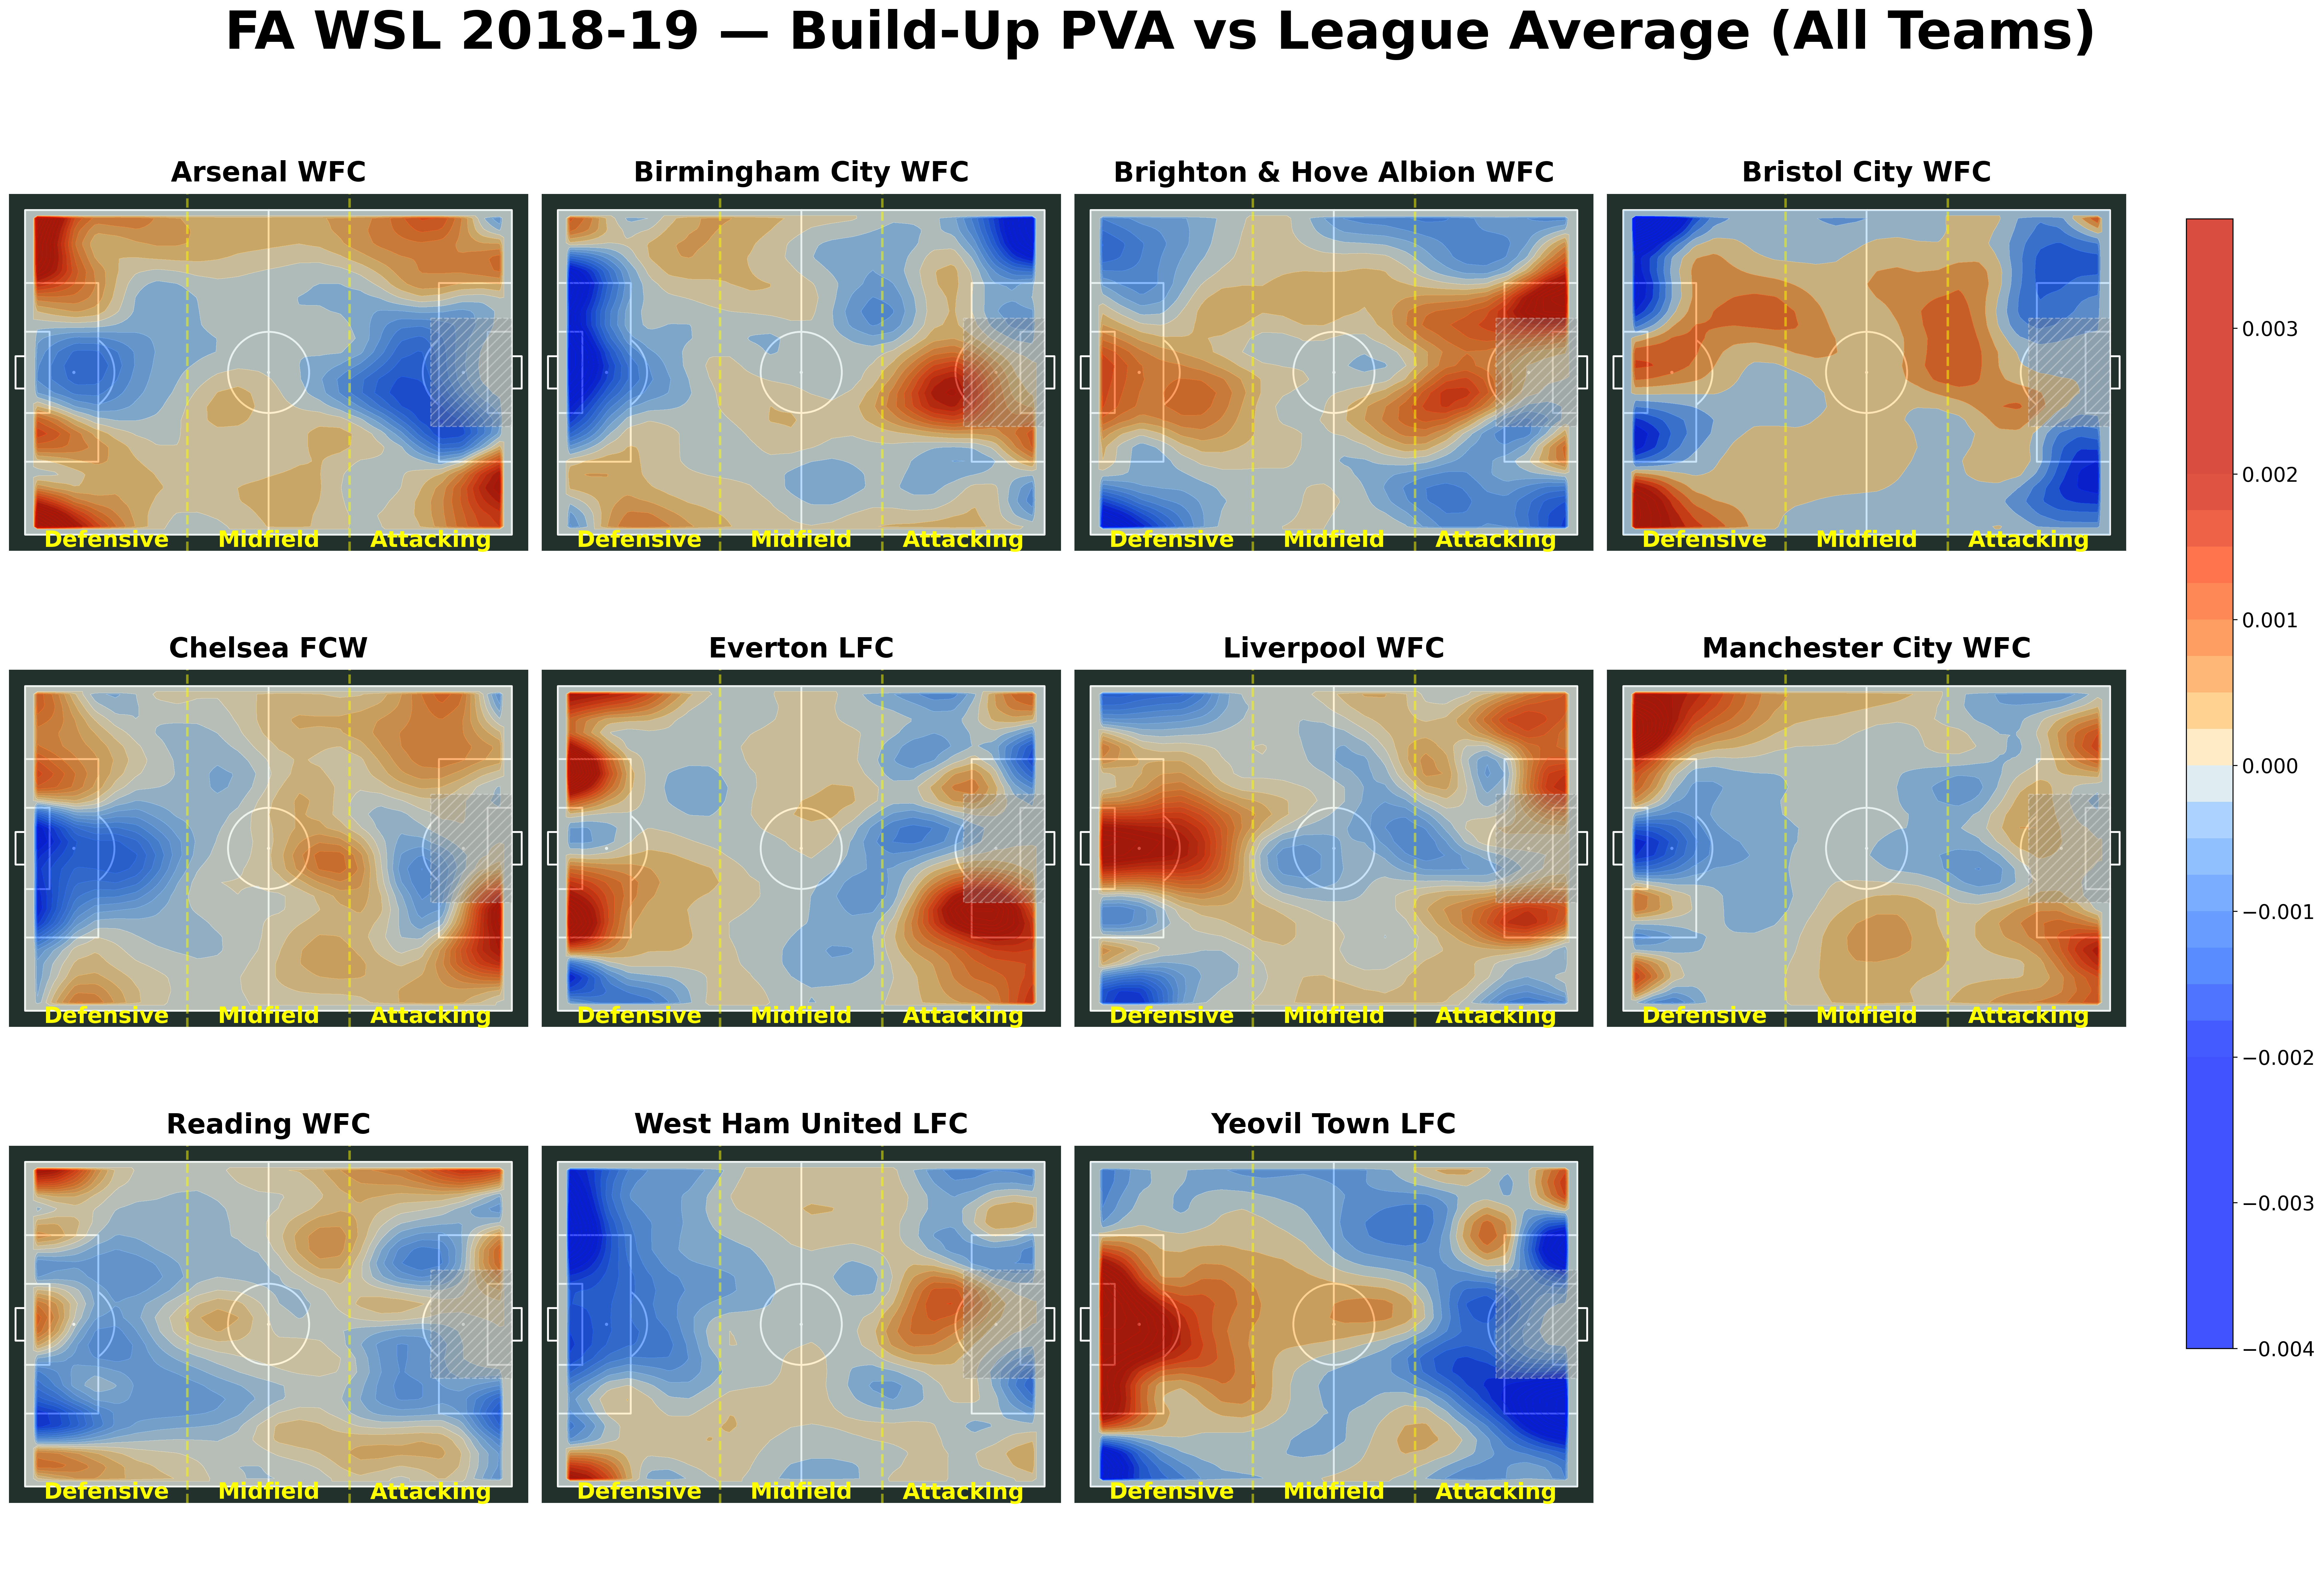
\includegraphics[width=\textwidth]{open-data/visualizations/zone_analysis/fa_wsl_2018-19/KDE/team_comparison_by_category/05_all_teams_buildup_vs_league_avg.png}
    \caption{KDE. The same data smoothed across continuous space using kernel density estimation.}
    \label{fig:buildup_kde}
\end{subfigure}
\caption{PVA relative to league average for each team in the FA WSL 2018--19. This is defined as "buildup PVA" as it excludes actions in the danger zone. Warm colors (red/orange) indicate zones where the team's mean PVA is above the league average whereas cool colors (blue) indicate zones where it falls below.}
\label{fig:buildup_both}
\end{figure}

\subsubsection{Zone Value Added (RQ3)}

Table~\ref{tab:zva} presents the league table for 2018--19, sorted by mean PVA per action, and alongside includes the ZVA/Action as well as the ZVA \% of PVA. ZVA quantifies how much value each team gains or loses based on where they distribute their actions, using league-average zone values.

\begin{table}[H]
\centering
\caption{FA WSL 2018--19 league table sorted by mean PVA per action, with ZVA. ZVA uses league-average PVA in each zone to measure the value gained or lost from spatial allocation.}
\label{tab:zva}
\begin{tabular}{clccc}
\toprule
\textbf{\#} & \textbf{Team} & \textbf{PVA/Action} & \textbf{ZVA/Action} & \textbf{ZVA \% of PVA} \\
\midrule
1  & Arsenal WFC             & 0.00255 & +0.00069 & +26.9\% \\
2  & Chelsea FCW              & 0.00254 & +0.00053 & +20.8\% \\
3  & Manchester City WFC      & 0.00240 & +0.00017 & +7.1\% \\
4  & Yeovil Town LFC          & 0.00209 & $-$0.00022 & $-$10.5\% \\
5  & Liverpool WFC            & 0.00207 & $-$0.00030 & $-$14.4\% \\
6  & Everton LFC              & 0.00202 & $-$0.00013 & $-$6.3\% \\
7  & Reading WFC              & 0.00201 & +0.00004 & +2.1\% \\
8  & West Ham United LFC      & 0.00195 & $-$0.00005 & $-$2.3\% \\
9  & Brighton \& Hove Albion  & 0.00186 & $-$0.00016 & $-$8.8\% \\
10 & Bristol City WFC         & 0.00182 & $-$0.00021 & $-$11.4\% \\
11 & Birmingham City WFC      & 0.00166 & $-$0.00037 & $-$22.5\% \\
\bottomrule
\end{tabular}
\end{table}

Arsenal's ZVA accounts for +26.9\% of their mean PVA. This means that over a quarter of their per-action value is explained by the fact that they distribute more actions into zones that carry high league-average value. At the other end of the table, Birmingham City's ZVA is $-$22.5\%, meaning their zone distribution tilts toward lower value zones, reducing their PVA relative to what league-average allocation would produce. The same pattern holds in 2020--21, where Arsenal (+16.5\%), Chelsea (+18.3\%), and Manchester City (+13.2\%) have positive ZVA, while Birmingham ($-$24.5\%) and Tottenham ($-$22.7\%) have negative ZVA.

Removing ZVA from each team's PVA reshuffles the league table substantially. Arsenal drops from 1st to 11th (last), and Chelsea falls from 2nd to 8th, indicating that much of their PVA advantage comes from \emph{where} they play rather than \emph{how well} they execute within each zone. Conversely, Liverpool rises from 5th to 1st, Birmingham climbs from 11th to 5th, and Bristol City moves from 10th to 5th, suggesting these teams are penalized by an unfavorable spatial allocation.

Figure~\ref{fig:zva_facet} visualizes the per-zone ZVA contribution for each team, showing which zones drive positive or negative spatial value.

\begin{figure}[H]
\centering
\begin{subfigure}[b]{\textwidth}
    \centering
    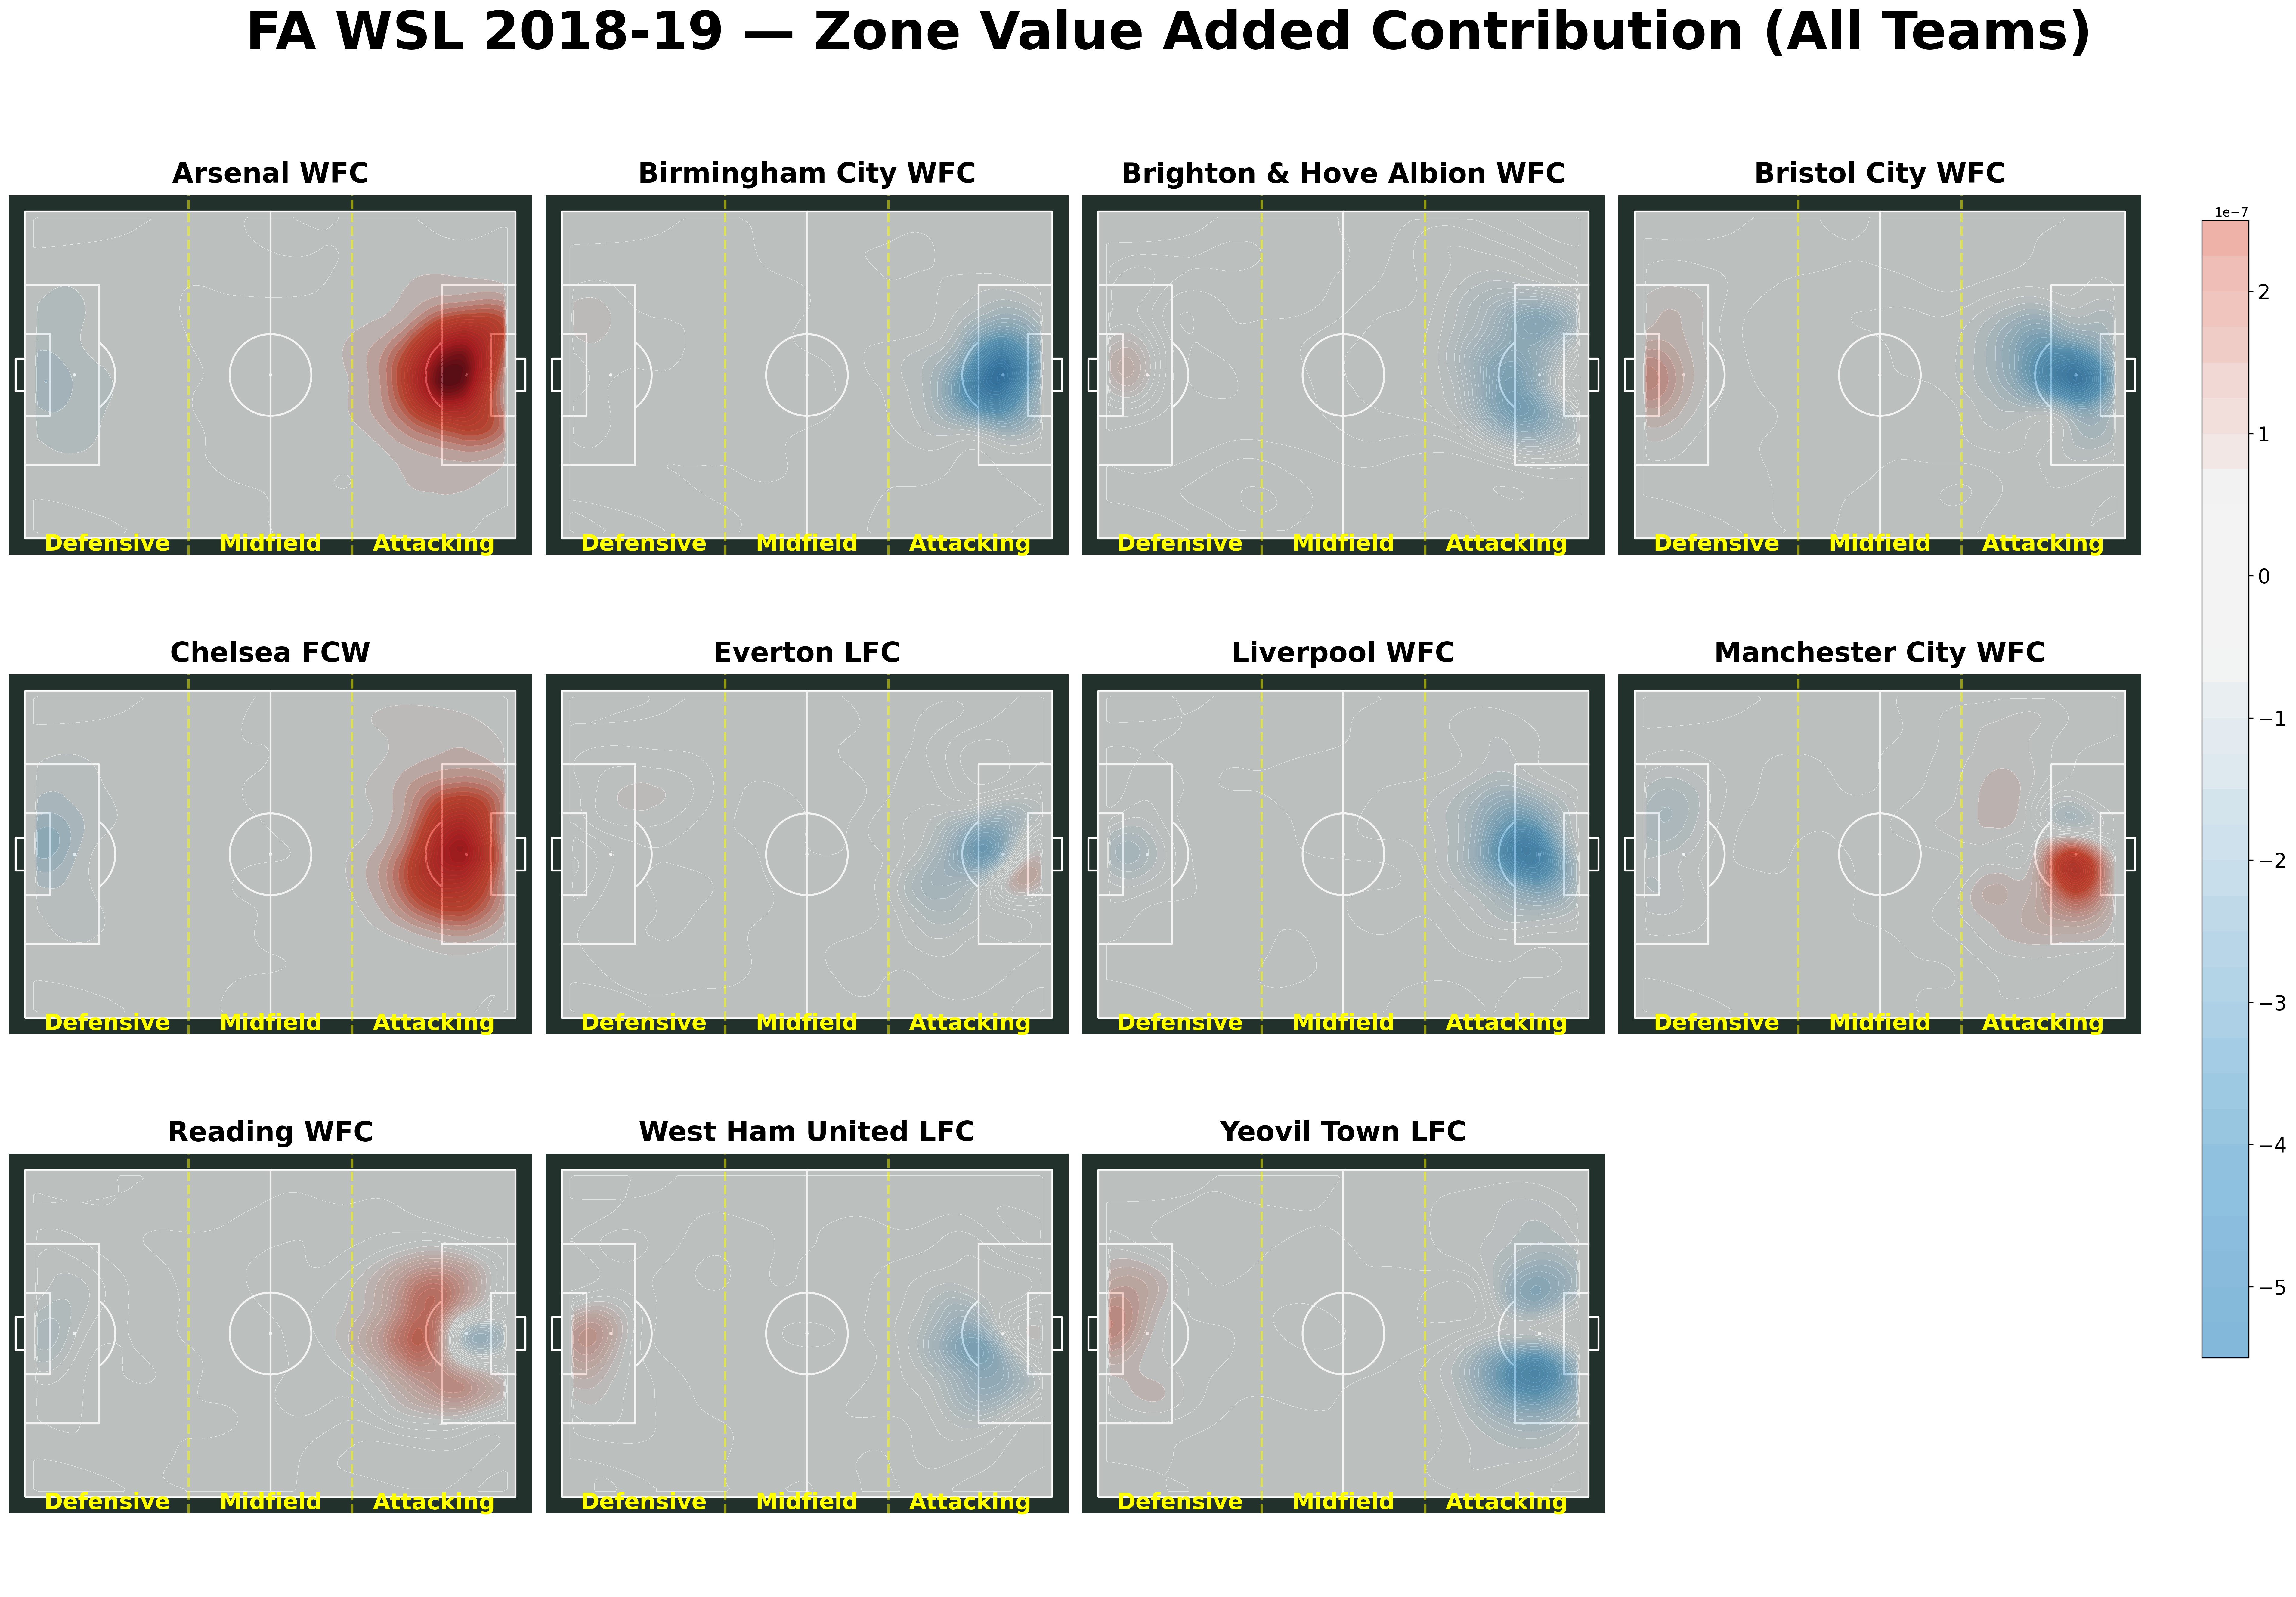
\includegraphics[width=\textwidth]{open-data/visualizations/zone_analysis/fa_wsl_2018-19/KDE/team_comparison_by_category/06_all_teams_zva_contribution.png}
    \caption{ZVA contribution across all zones.}
    \label{fig:zva_all}
\end{subfigure}

\vspace{0.5em}

\begin{subfigure}[b]{\textwidth}
    \centering
    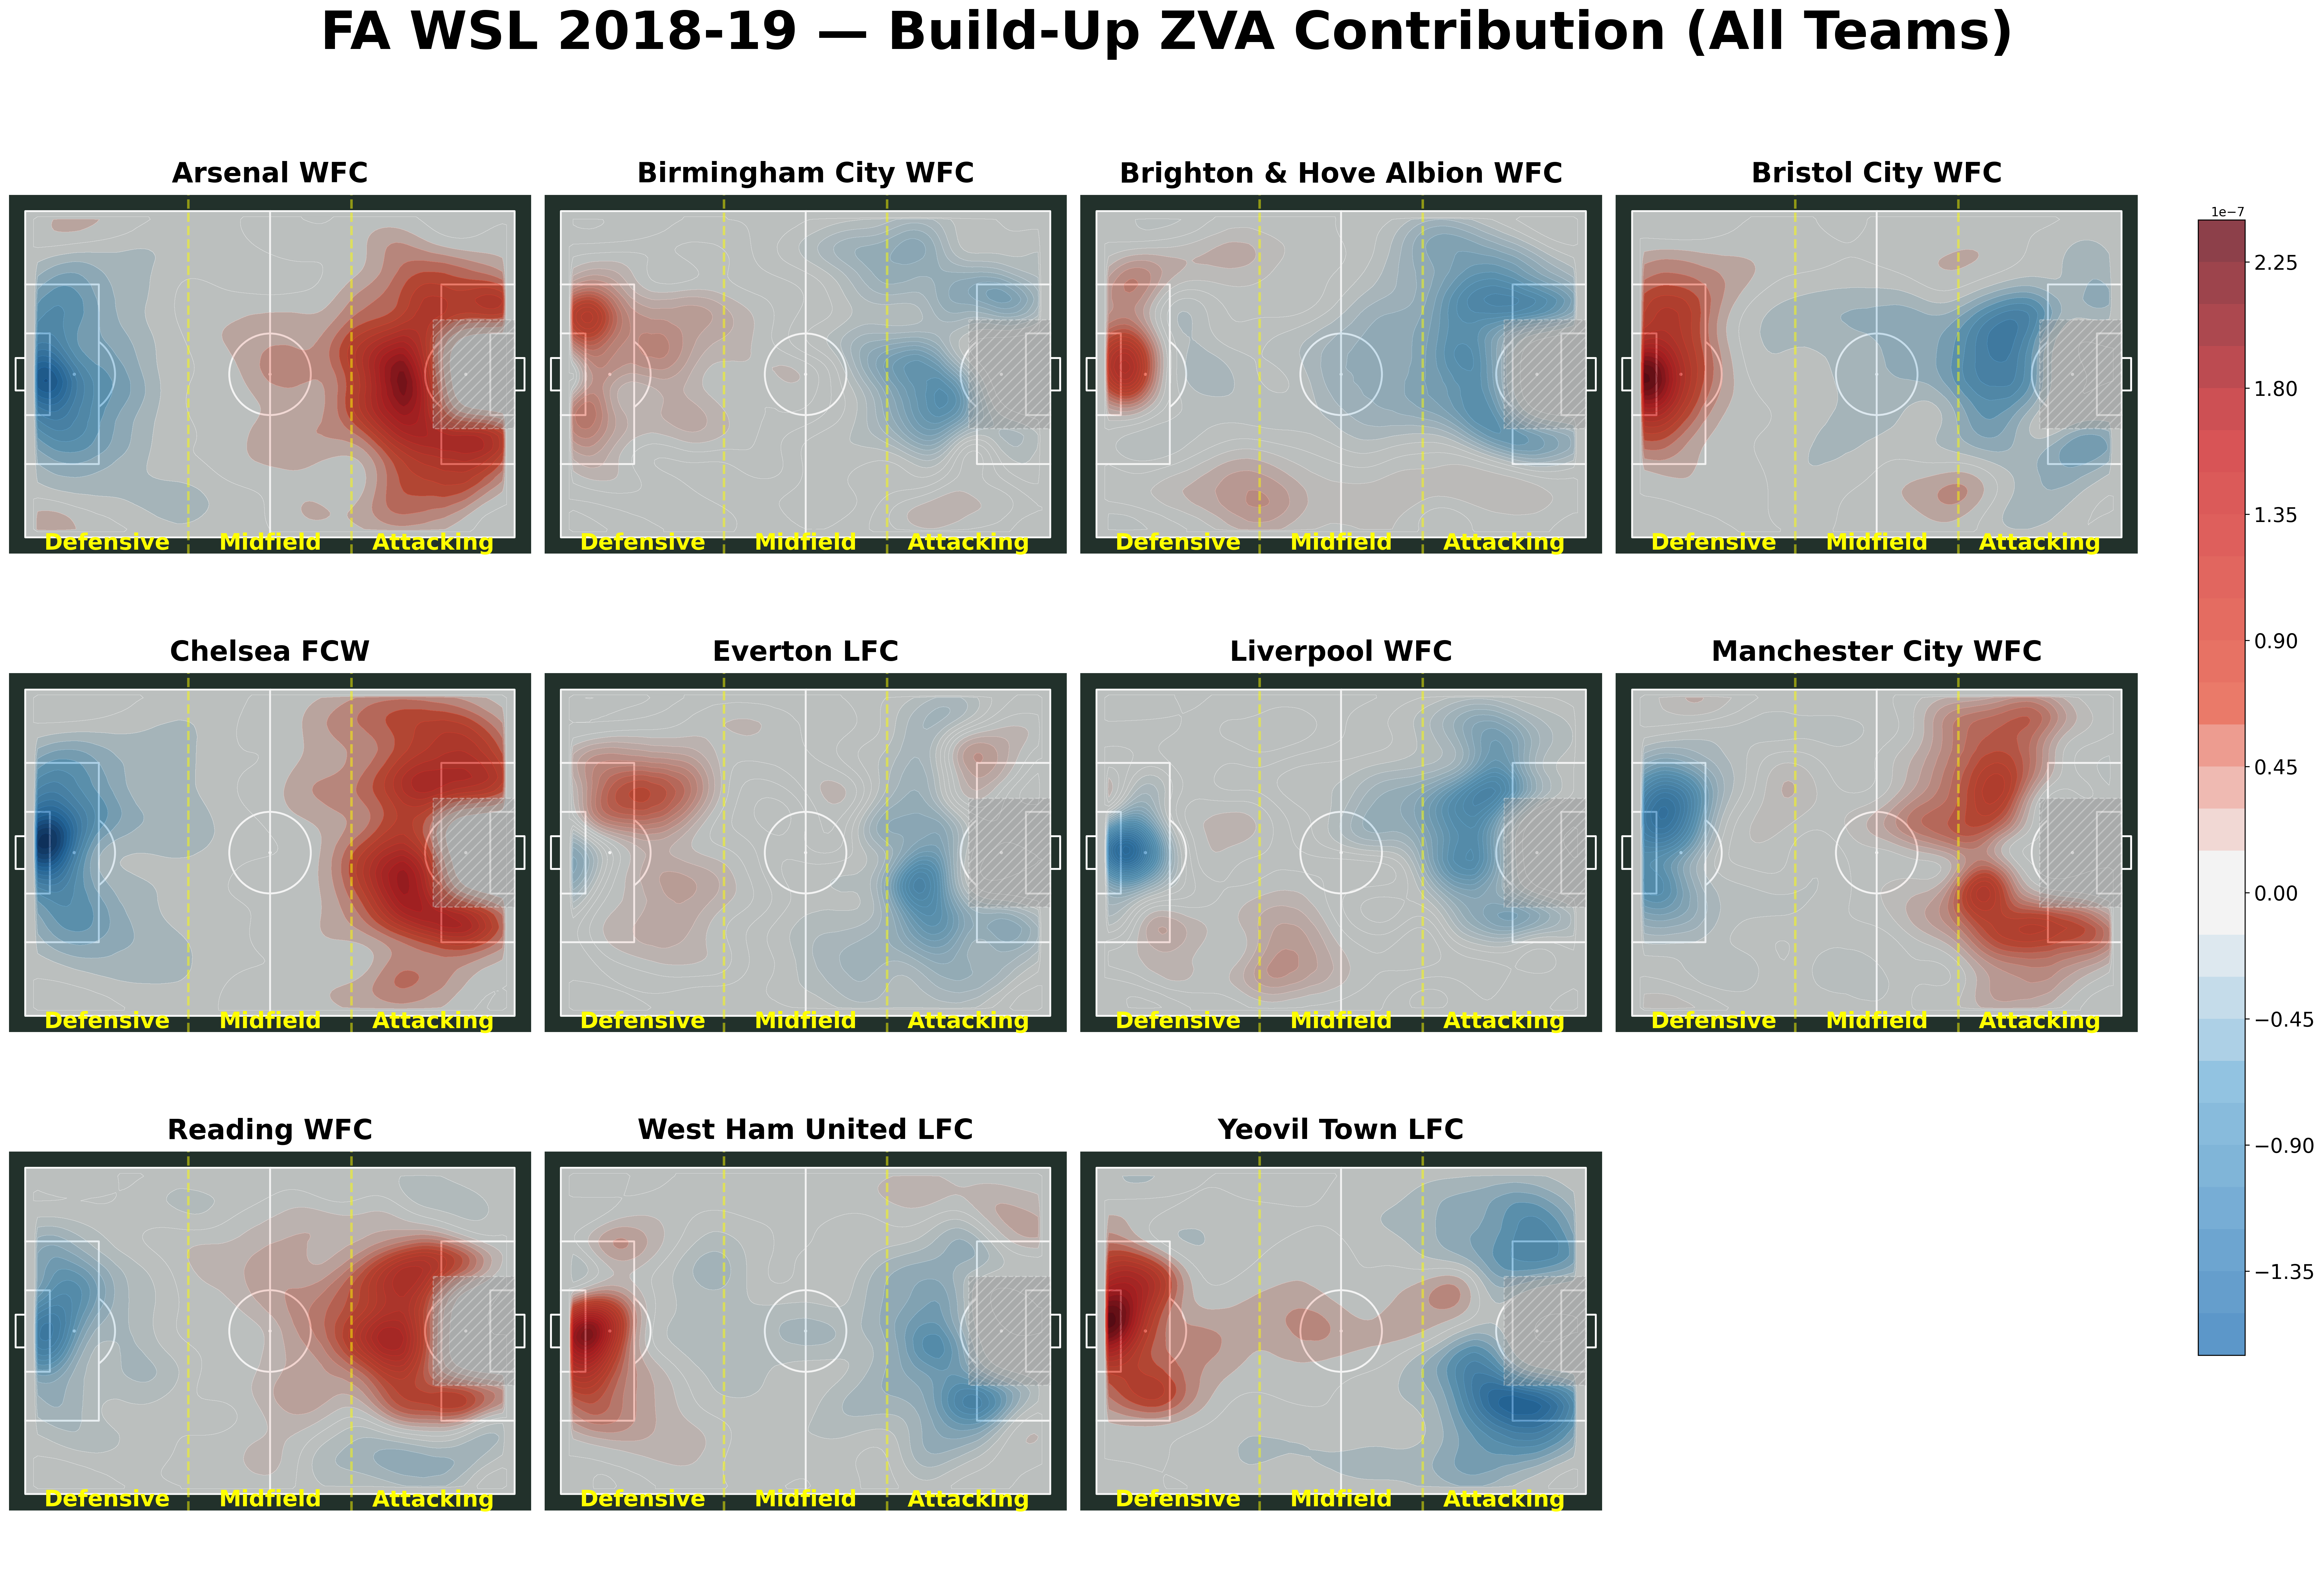
\includegraphics[width=\textwidth]{open-data/visualizations/zone_analysis/fa_wsl_2018-19/KDE/team_comparison_by_category/07_all_teams_zva_buildup.png}
    \caption{ZVA contribution from buildup zones only (danger zone excluded).}
    \label{fig:zva_buildup}
\end{subfigure}
\caption{Zone-level ZVA contribution (KDE) for each team in the FA WSL 2018--19. Red zones contribute positively to ZVA (team over-utilizes a zone with positive league-average PVA); blue zones contribute negatively (team over-utilizes a zone with negative league-average PVA, or under-utilizes a positive one).}
\label{fig:zva_facet}
\end{figure}

\paragraph{The Confounding Problem.}

While ZVA appears to be a powerful metric, a critical caveat accompanies it. Team quality, while it is being partially accounted for through the LOO league PVA baseline, still ultimately confounds where a team \emph{can} play on the pitch. Arsenal illustrates this clearly. With ZVA, they rank 1st, but stripping ZVA from their PVA drops them to 11th. Because Arsenal is such a talented team, they can sustain possession in high-value zones, inflating their ZVA. Weaker teams are unable to access these high-value zones and may be forced to play in their defensive third not by choice but by opponent pressure and talent level. In other words, while ZVA does account for how well teams are able to access certain zones of the pitch, it cannot distinguish whether a team's spatial allocation reflects true tactical optimization or simply the zone access that comes with team quality. A more fitting interpretation of Arsenal's +26.9 ZVA \% PVA is that their \emph{ability} to play in high-value zones, rather than strictly their \emph{choice} to route their actions through these zones is what explains ${\sim}27\%$ of their total team PVA. While interesting in its own right, this is not as strong as claiming that Arsenal's \emph{choice} to play in these zones accounts for 27\% of their PVA, and therefore motivates the possession-patterning analysis in the next section, which examines entire possession-routing decisions starting from each phase of play (defensive third, midfield, attacking third), rather than just the spatial distribution of individual actions. 

These results address RQ3: zone distribution explains a substantial share of a team's mean PVA (up to 27\%), though the metric is heavily confounded by team quality and reflects zone accessibility as much as tactical choice.

% --------------------------------------------------------------------------
\subsection{Possession Patterning}

\subsubsection{Clustering Results}

Through route-scouting and stratified $k$-medoids clustering we identify 18 patterns starting in the defensive-third, 18 starting in the midfield, and 9 attacking-third patterns (45 total). Approximately 25\% of possessions in each stratum are unassigned (distance to nearest medoid exceeds the 75th percentile), which improves the quality of the assigned clusters.

Figure~\ref{fig:clusters} shows the clustered, possession-pattern routes, organized by starting third.

\begin{figure}[H]
\centering
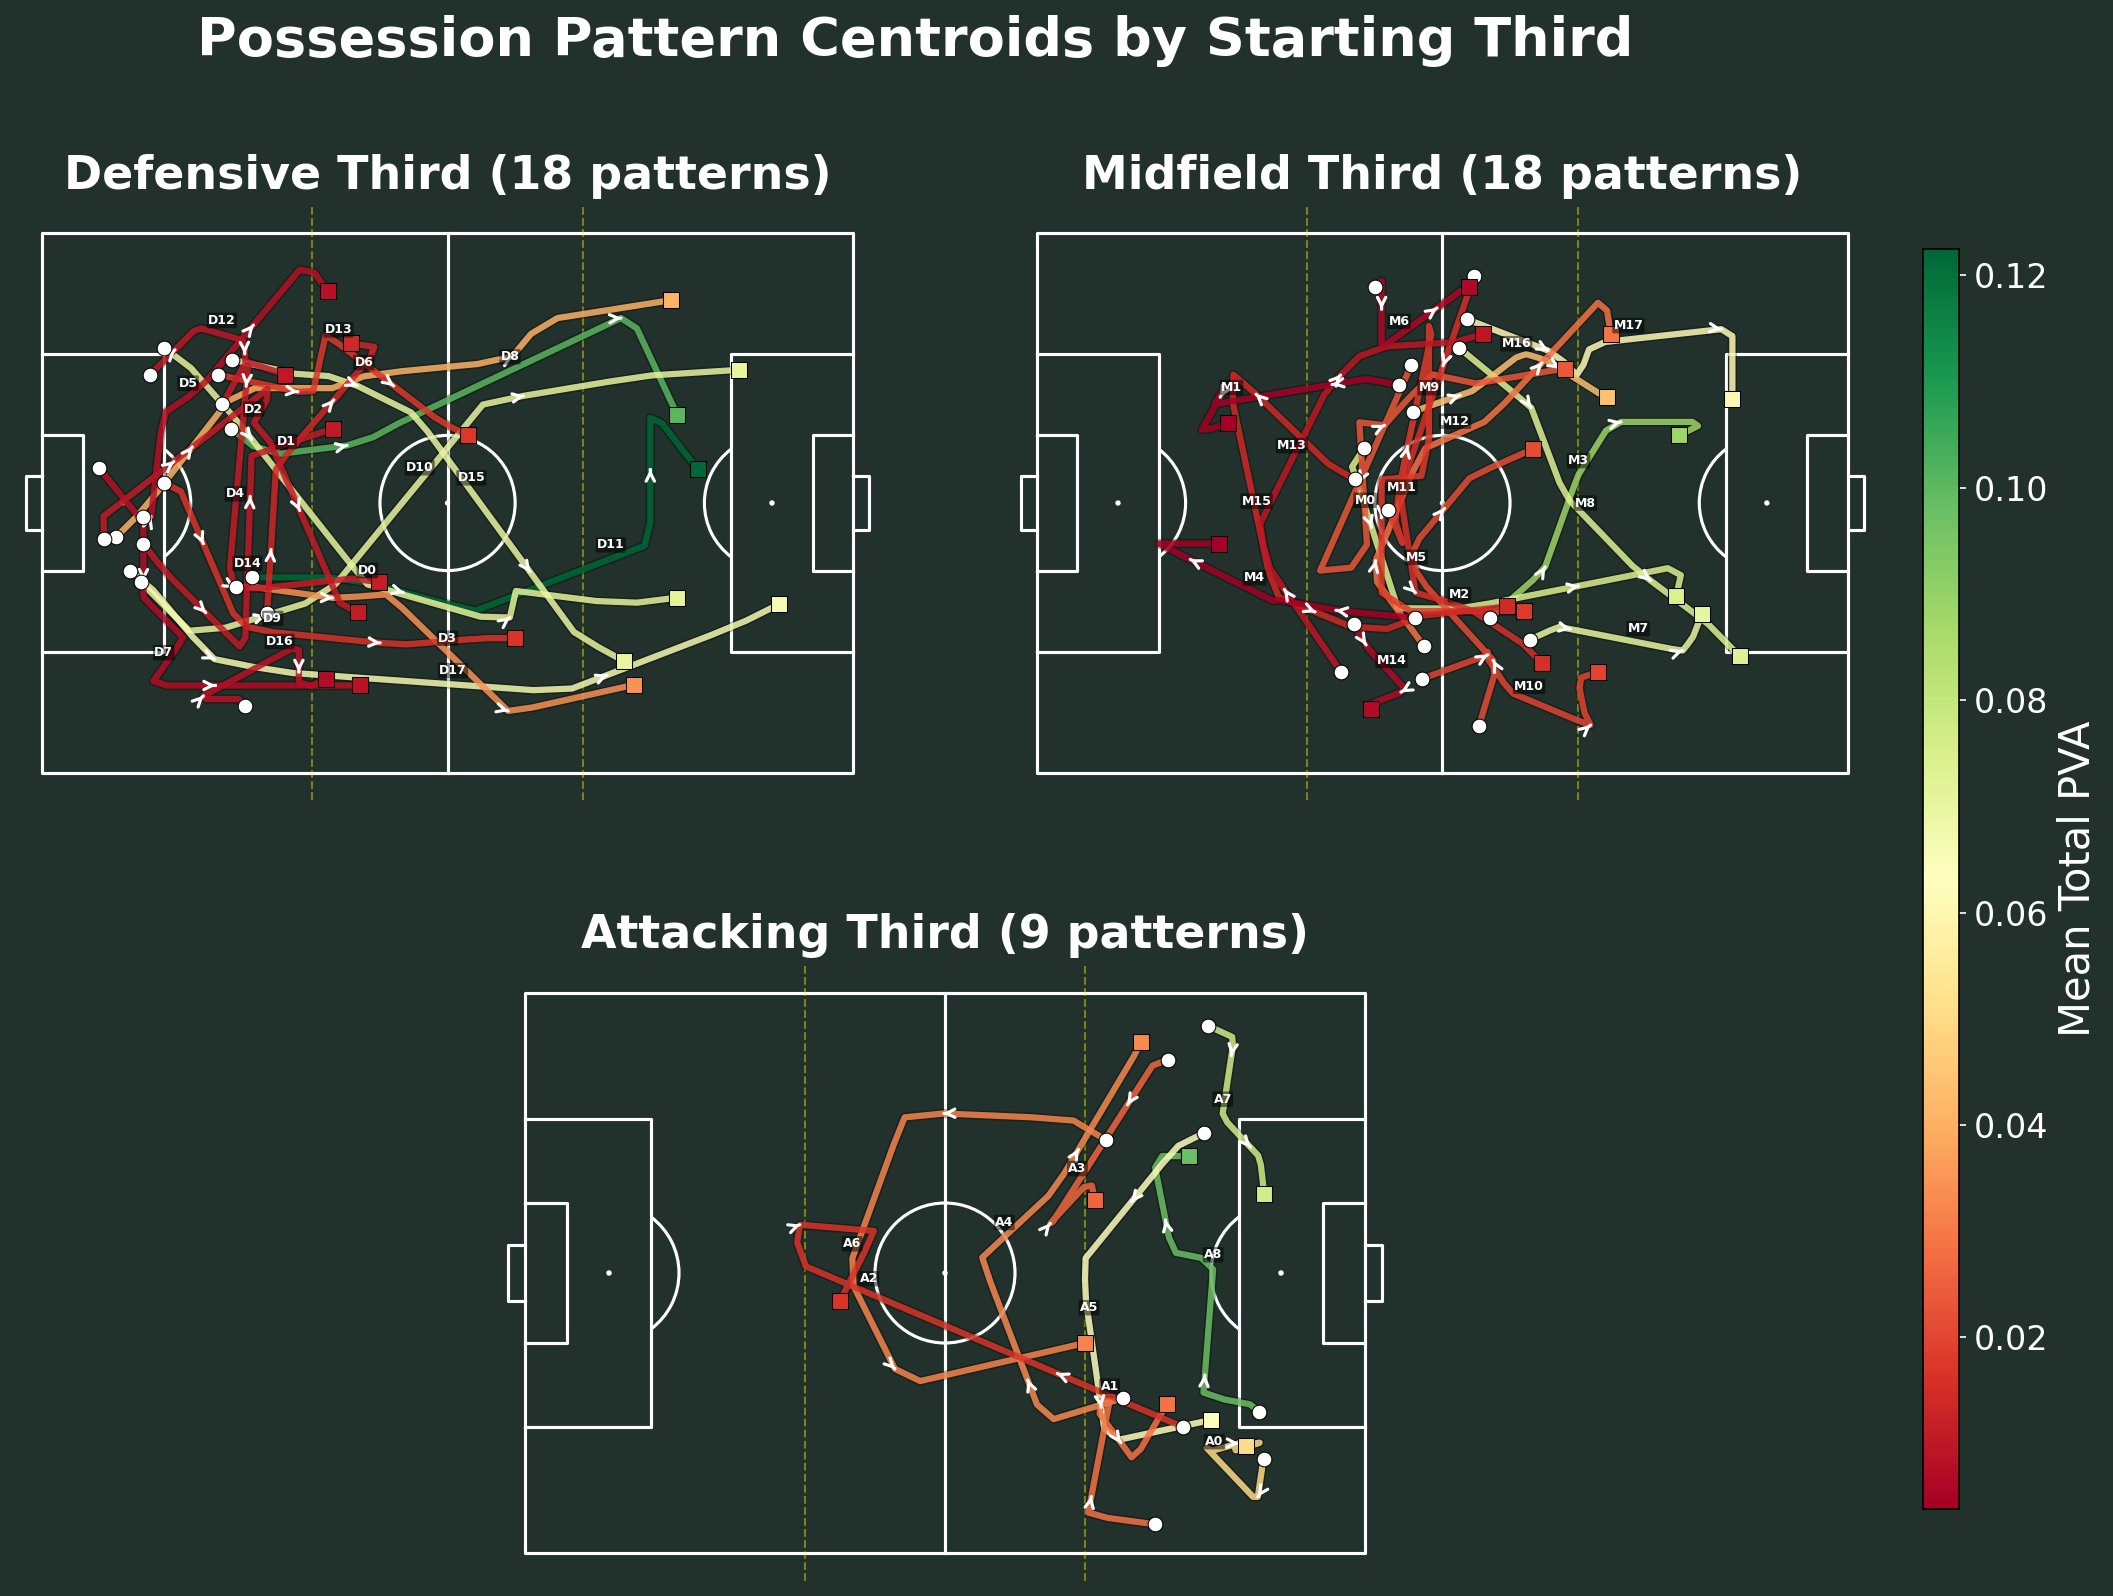
\includegraphics[width=\textwidth]{cluster_centroids_all.png}
\caption{Cluster medoid routes for all 45 possession patterns, organized by starting third (defensive, midfield, attacking). Each route represents the spatial trajectory of a typical possession in that cluster.}
\label{fig:clusters}
\end{figure}

\subsubsection{Possession-Level Performance Differences}

Figures~\ref{fig:poss_perf_arsenal} and~\ref{fig:poss_perf_birmingham} display each team's 45 cluster patterns individually, showing the medoid route for each cluster alongside the team's usage percentage and the difference between the team's mean PVA and the league-average PVA for that pattern. Red patterns indicate clusters where the team outperforms the league average; blue patterns indicate underperformance. This grid format allows analysts and coaches alike to identify exactly which possession types a team executes well and which represent areas for improvement.

Arsenal's grid (Figure~\ref{fig:poss_perf_arsenal}) has more red and neutral patterns, reflecting better overall execution than Birmingham, whose grid (Figure~\ref{fig:poss_perf_birmingham}), by contrast, shows a more mixed profile with several blue patterns, particularly those at the top of the grid that have a greater league average PVA associated with them.

\begin{figure}[H]
\centering
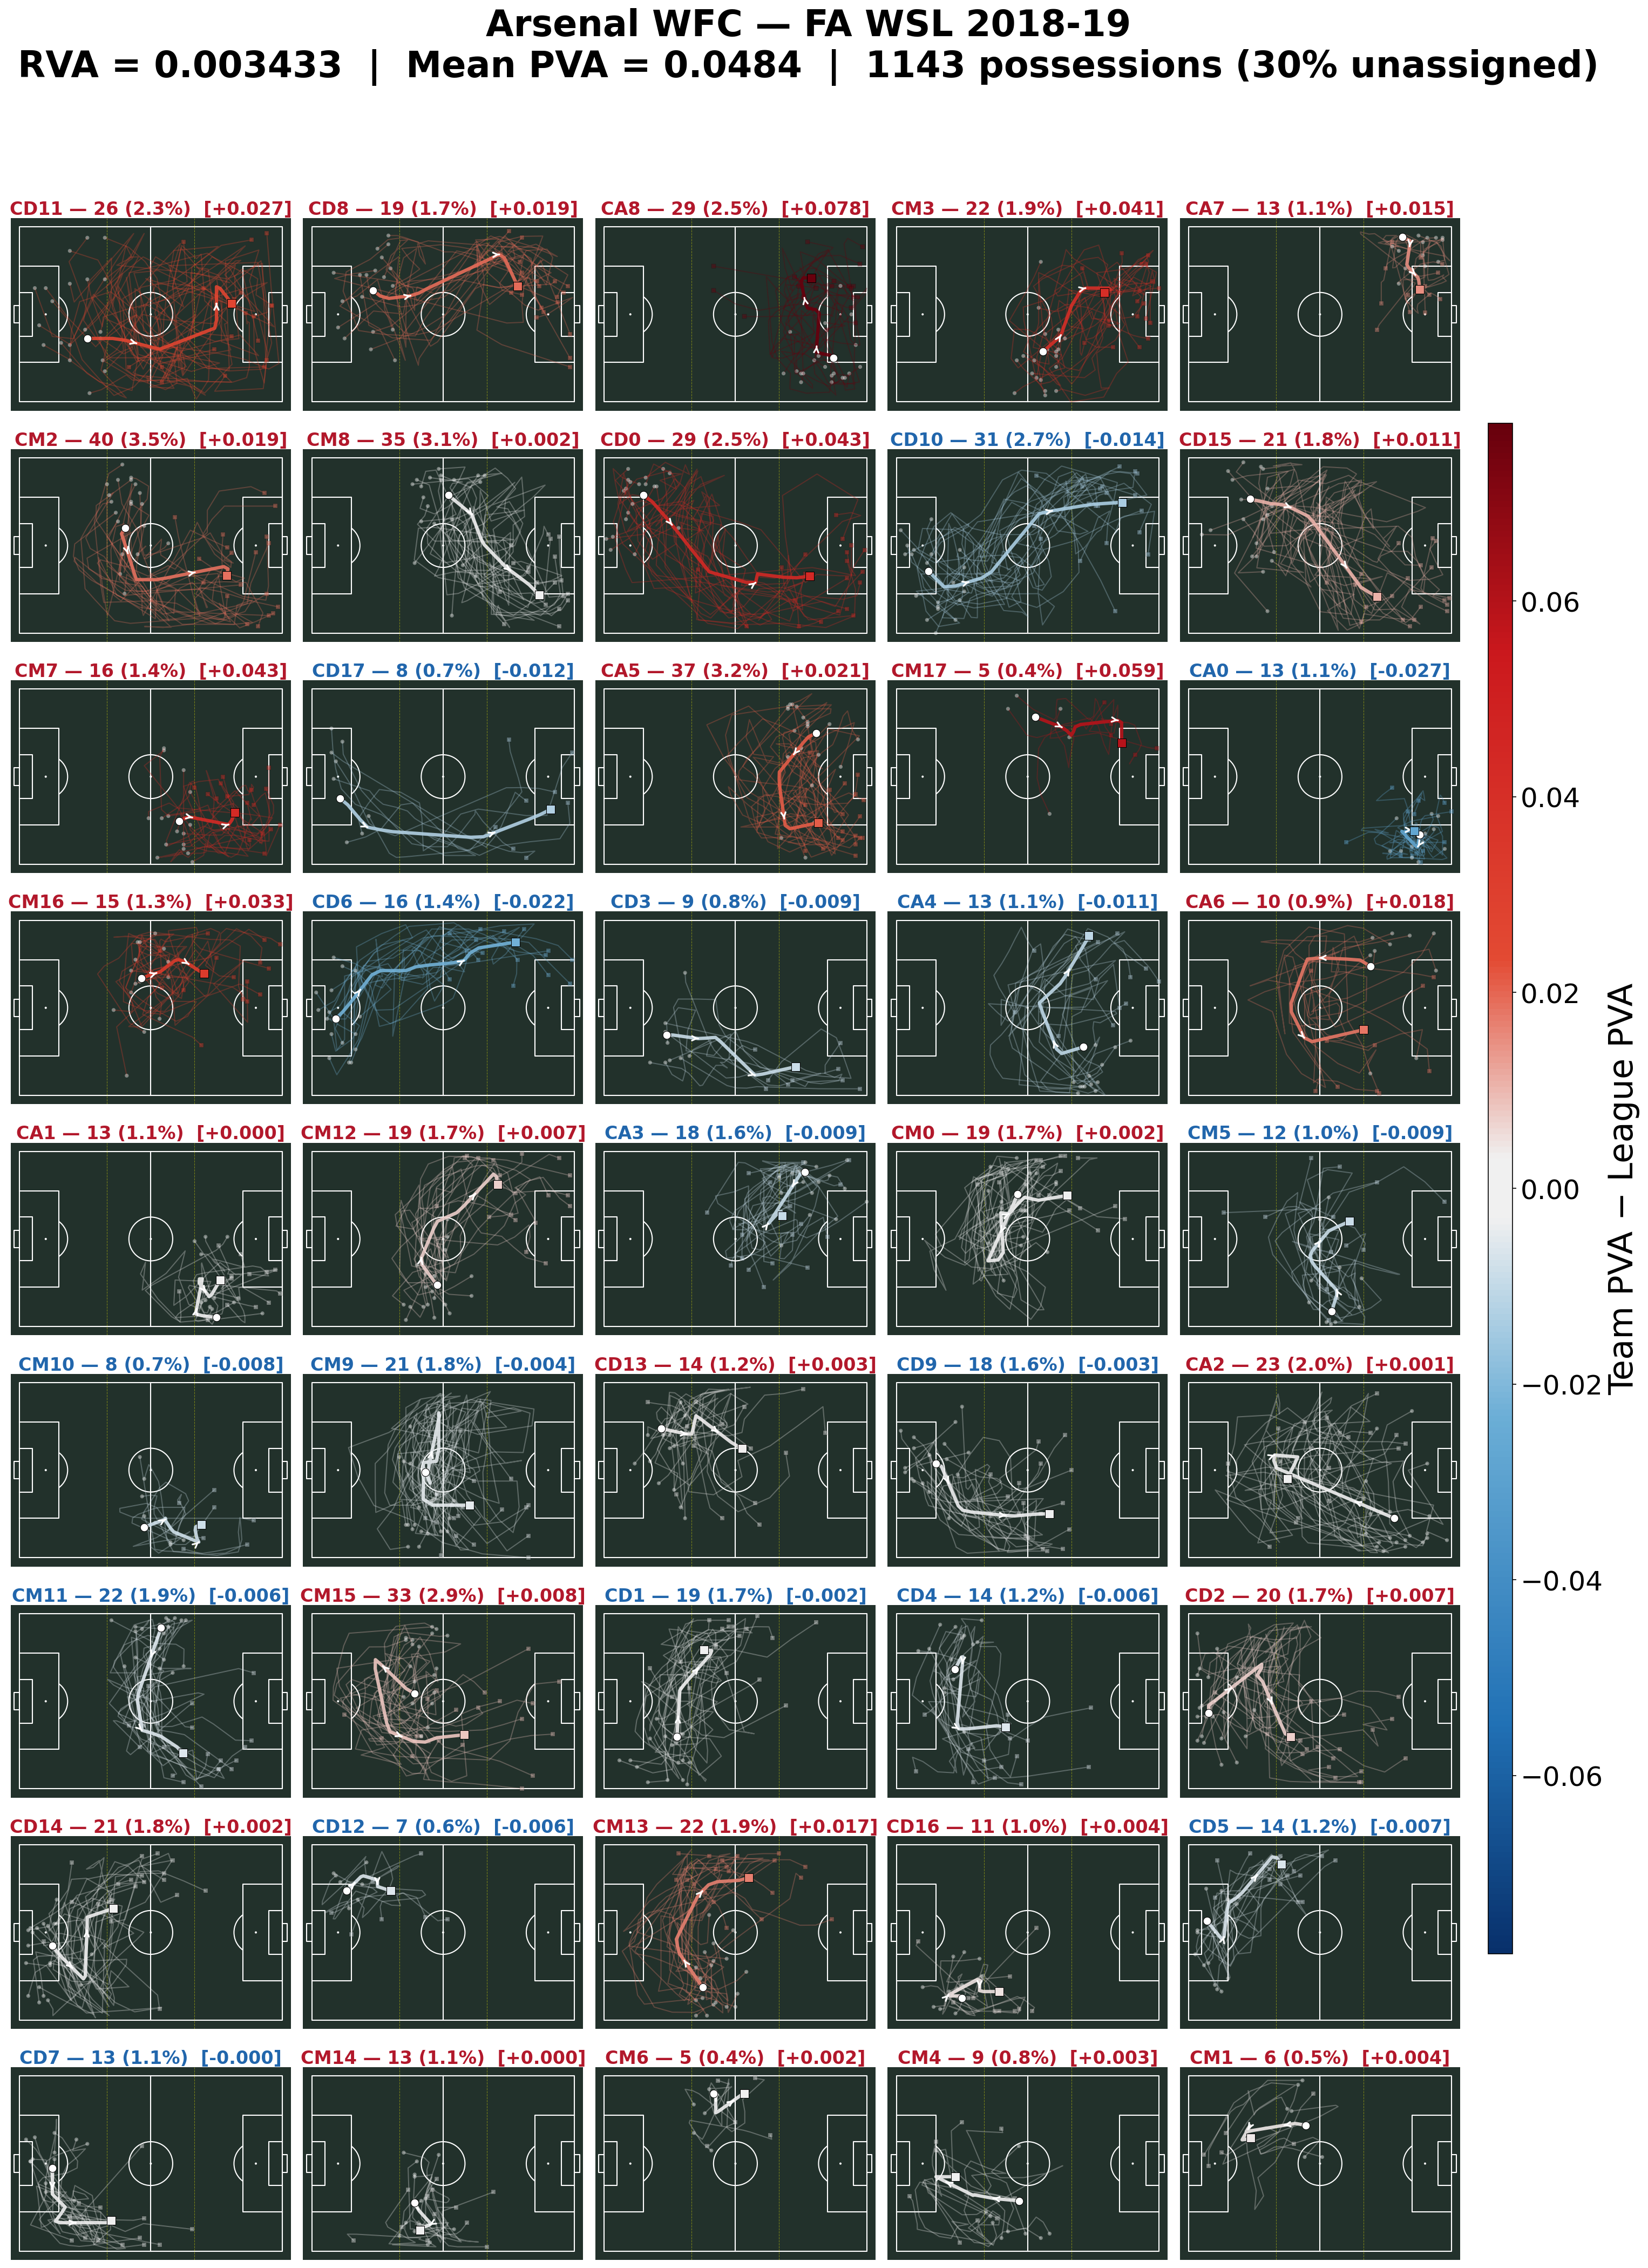
\includegraphics[width=\textwidth]{open-data/visualizations/possession_patterning_analysis/teams/wsl_2018-19_arsenal_wfc/pattern_usage_grid.png}
\caption{Pattern usage and performance grid for Arsenal WFC (FA WSL 2018--19). Each subplot shows a cluster's medoid route, the team's usage percentage, and is colored by Team PVA $-$ League PVA. Red indicates the team outperforms the league average on that pattern; blue indicates underperformance.}
\label{fig:poss_perf_arsenal}
\end{figure}

\begin{figure}[H]
\centering
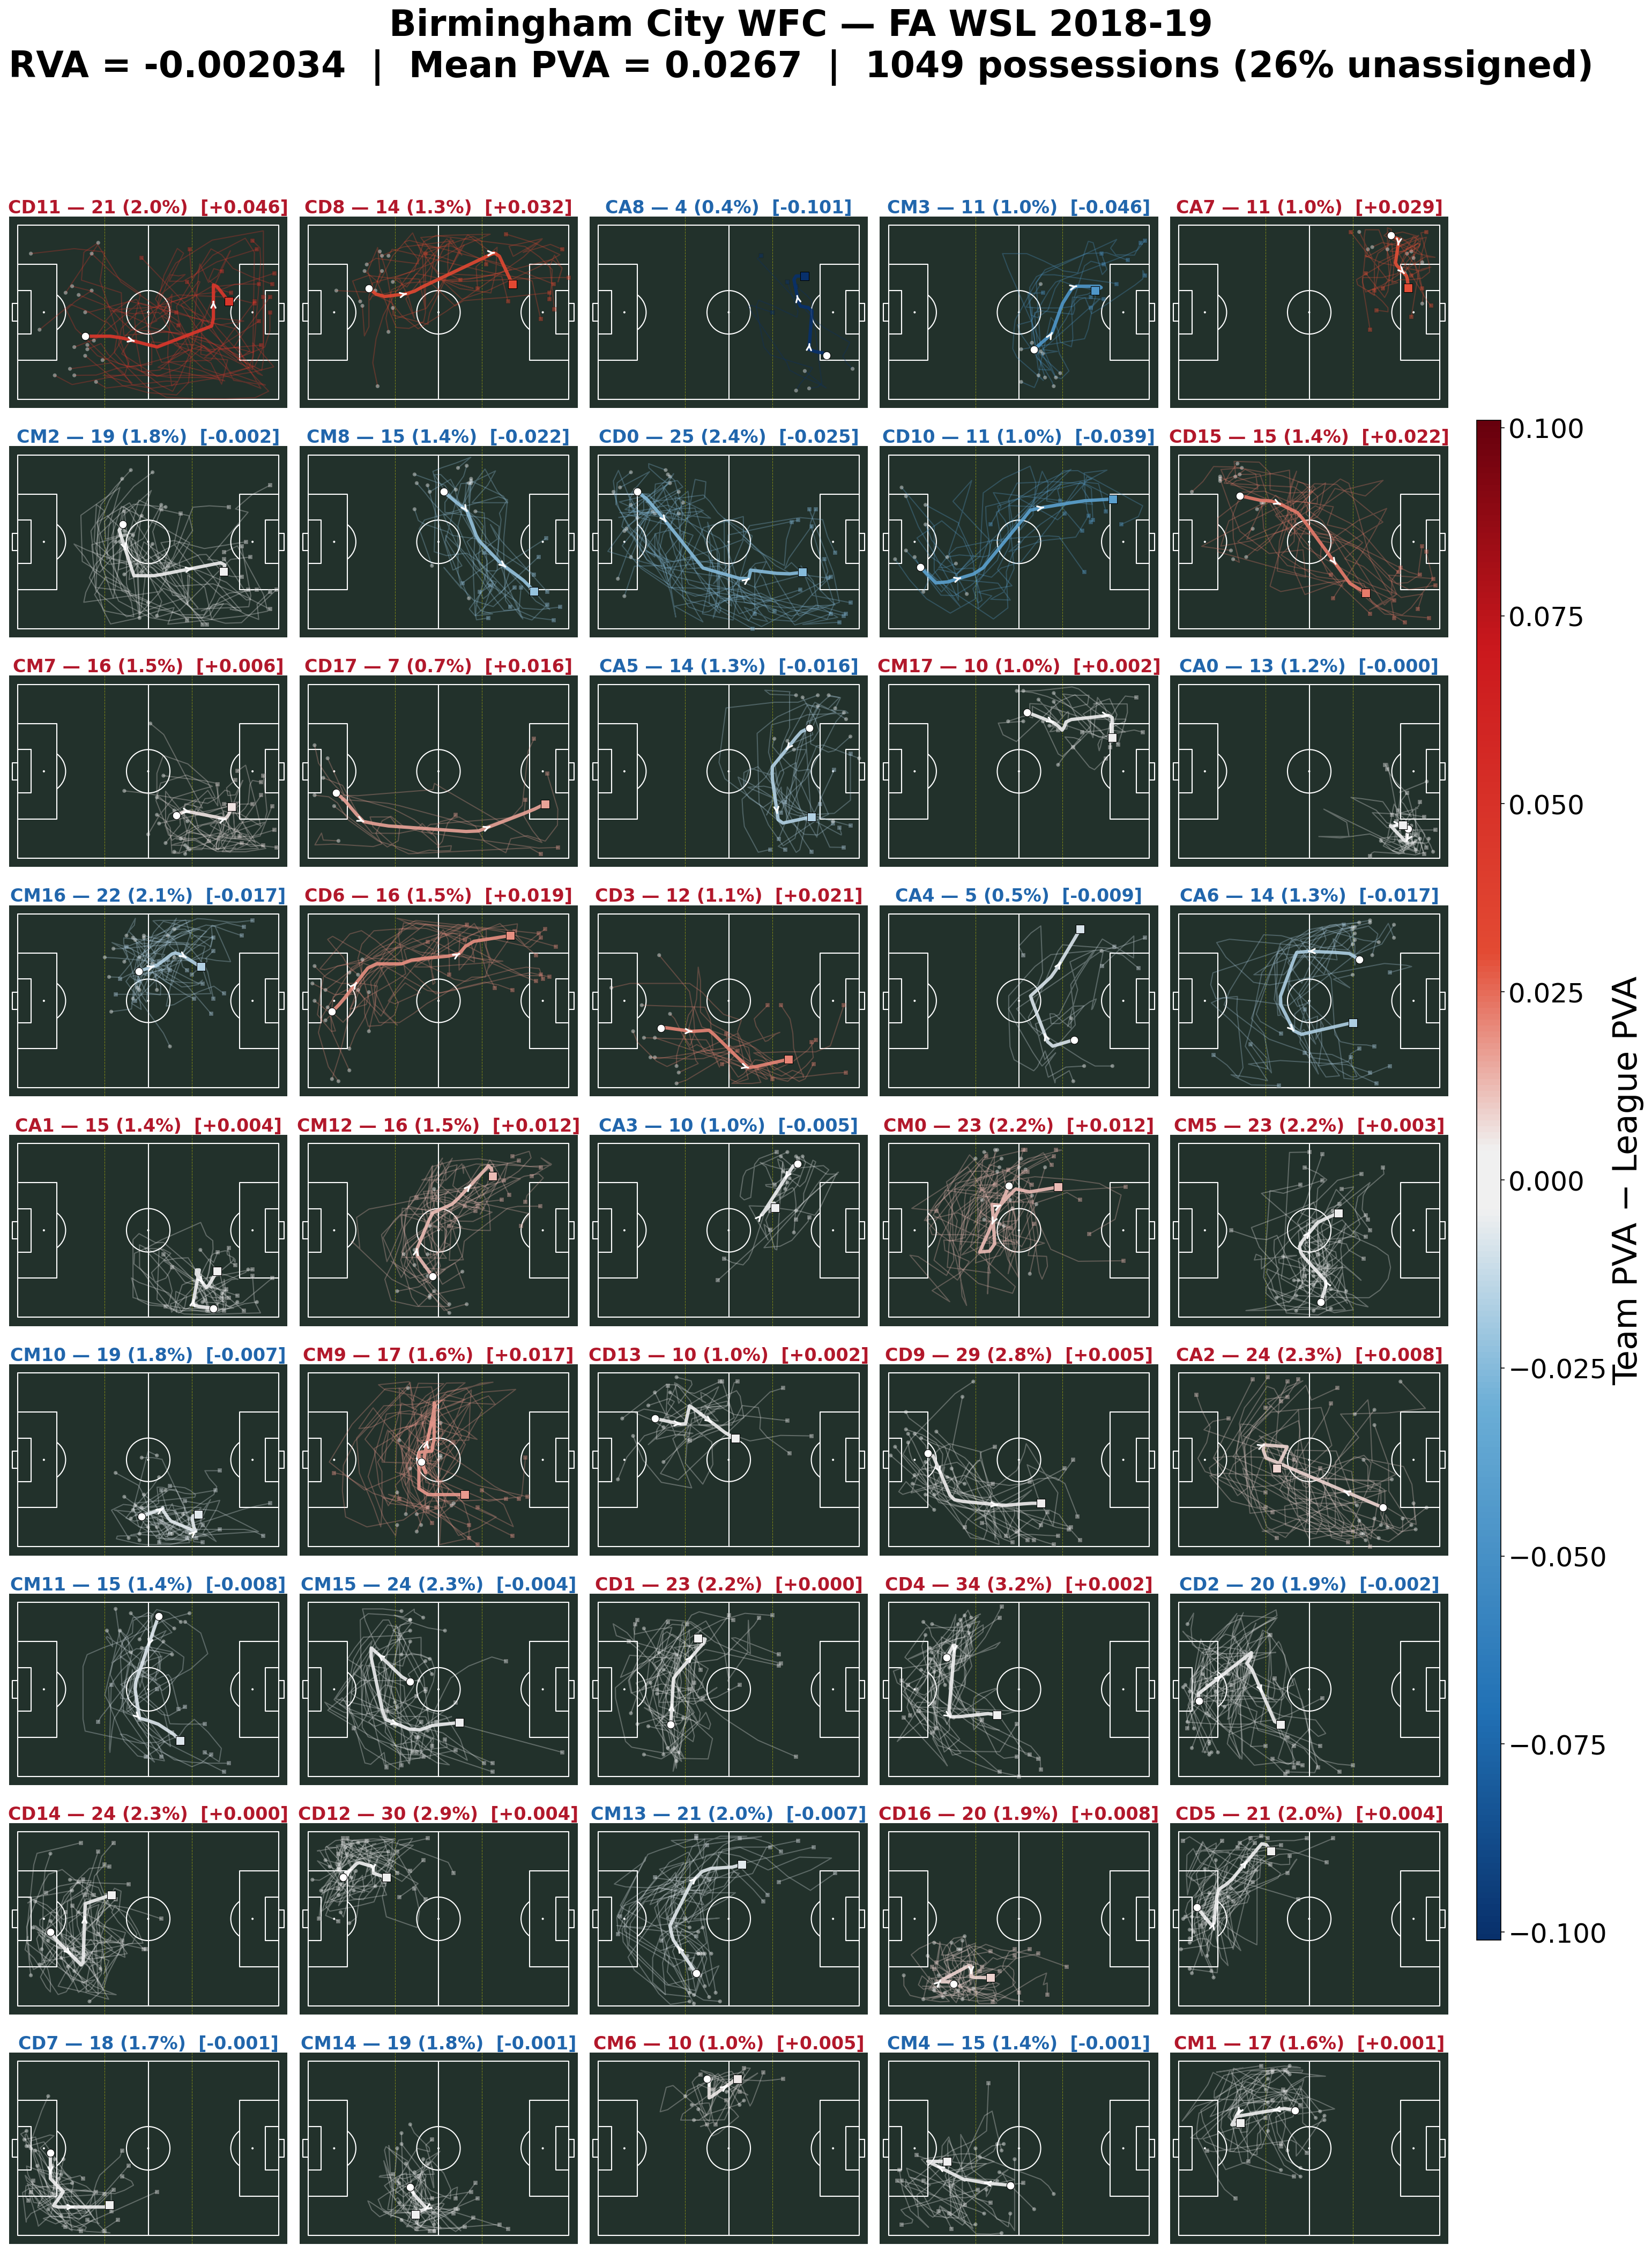
\includegraphics[width=\textwidth]{open-data/visualizations/possession_patterning_analysis/teams/wsl_2018-19_birmingham_city_wfc/pattern_usage_grid.png}
\caption{Pattern usage and performance grid for Birmingham City WFC (FA WSL 2018--19). Same format as Figure~\ref{fig:poss_perf_arsenal}. Birmingham shows a more mixed profile with more blue (underperforming) patterns.}
\label{fig:poss_perf_birmingham}
\end{figure}

\subsubsection{Routing Value Added (RQ4)}

Table~\ref{tab:rva} presents the league table for 2018--19, sorted by mean PVA per possession. Shown alongside are RVA per possession, RVA \% of PVA, PVA rank (raw), PVA rank without RVA, and the resulting rank change. RVA quantifies how much value each team gains or loses based on which possession patterns they favor, using league-average pattern values.

\begin{table}[H]
\centering
\caption{FA WSL 2018--19 league table sorted by mean PVA per possession. Columns show RVA per possession, RVA as a percentage of PVA, the team's raw PVA rank, where each team would rank without RVA, and the resulting rank change ($\Delta$).}
\label{tab:rva}
\begin{tabular}{clcccccc}
\toprule
\textbf{\#} & \textbf{Team} & \textbf{PVA} & \textbf{RVA} & \textbf{RVA \%} & \textbf{Rank} & \textbf{w/o} & $\boldsymbol{\Delta}$ \\
\midrule
1  & Arsenal WFC         & 0.048 & +0.003 & +7.1\%  & 1  & 1  & --- \\
2  & Chelsea FCW          & 0.043 & +0.002 & +3.5\%  & 2  & 2  & --- \\
3  & Manchester City WFC  & 0.036 & +0.001 & +4.0\%  & 3  & 3  & --- \\
4  & Reading WFC          & 0.030 & +0.002 & +7.2\%  & 4  & 7  & +3 \\
5  & Everton LFC          & 0.029 & +0.000 & +1.1\%  & 5  & 5  & --- \\
6  & Liverpool WFC        & 0.029 & +0.002 & +6.4\%  & 6  & 8  & +2 \\
7  & West Ham United LFC  & 0.028 & $-$0.001 & $-$1.9\% & 7  & 6  & $-$1 \\
8  & Birmingham City WFC  & 0.027 & $-$0.002 & $-$7.6\% & 8  & 4  & $-$4 \\
9  & Brighton \& Hove Albion & 0.025 & +0.001 & +4.4\% & 9  & 9  & --- \\
10 & Bristol City WFC     & 0.021 & +0.002 & +9.7\%  & 10 & 10 & --- \\
11 & Yeovil Town LFC      & 0.021 & +0.003 & +14.4\% & 11 & 11 & --- \\
\bottomrule
\end{tabular}
\end{table}

RVA reveals notable ranking shifts among middle-of-the-table teams. Birmingham City WFC ranks 4th on execution quality alone (PVA minus RVA), but their negative routing patterns ($\text{RVA} = -0.002$) drag them to 8th in overall PVA, which is a four-place drop attributable to favoring lower-value possession routes and under-utilizing high-value ones. Conversely, Reading WFC would rank only 7th on execution quality, but favorable routing ($\text{RVA} = +0.002$) lifts them to 4th in overall PVA, which is a three-place rise. Liverpool WFC similarly gains two positions from favorable routing. The top three teams (Arsenal, Chelsea, Manchester City) maintain their positions regardless of routing effects, suggesting that for dominant teams, execution quality and talent outweigh routing decisions. This contrasts the ZVA findings, where removing ZVA dropped Arsenal from 1st to last. Furthermore, it reinforces the finding that the ZVA result was driven by the confounding between team quality and zone access. RVA's more modest ranking shifts suggest it better captures real tactical variation and nuance rather than being a proxy for team strength. 

These results address RQ4: routing patterns differ meaningfully in value, and RVA captures tactical nuance that ZVA cannot.

The 2020--21 season shows a similar pattern. RVA ranges from $-$0.0016 (Everton) to +0.0037 (Manchester United), with Manchester United's routing accounting for 9.2\% of their mean PVA. Bristol City (+11.7\%) and Birmingham (+14.5\%) show large positive RVA percentages despite being lower-ranked overall, suggesting that their routing decisions partially compensate for lower overall team strength.

\subsubsection{RVA by Phase of Play}

Breaking down RVA by starting third further reveals where routing advantages originate. In 2018--19, Arsenal's RVA is driven primarily by using routes starting in the defensive-third ($+0.0012$) and attacking-third routing ($+0.0014$), with a smaller midfield contribution ($+0.0008$). Birmingham's negative RVA is concentrated in midfield-third possessions ($-0.0016$), indicating that they tend to build up through lower value patterns when starting their possessions in the midfield. This breakdown suggests that RVA captures important tactical nuance that a zone grid approach cannot.

% ============================================================================
\section{Discussion}
% ============================================================================

\subsection{ZVA and RVA as Complementary Spatial Lenses}

ZVA and RVA evaluate spatial decisions at different levels. ZVA operates at the level of individual actions, asking how much value a team gains or loses from its distribution of actions across zones. RVA works at the level of full possessions and asks the analogous question for possession-routing patterns. Both apply the same value-added logic that compares a team's spatial allocation to a leave-one-out league baseline and weights by league-average values, but they capture different nuance. A team could have positive ZVA (its zone distribution favors high-value zones) but negative RVA (its possession routes favor low-value sequences), or vice versa.

The most relevant finding is how differently the two metrics shift the league table, when they are stripped from PVA. ZVA produces implausible ranking shifts (Arsenal 1st-to-last), highlighting ZVA as heavily confounded by team quality. RVA produces more realistic shifts (changes can be up to four positions). This contrast suggests that RVA captures genuine tactical variation and nuance, while ZVA largely reflects the zones a team can access given their overall team ability level. For middle-of-the-table teams, where overall team talent is similar, routing decisions appear to be a meaningful differentiator in determining how much value teams generate.

\subsection{Practical Implications}

Despite the confounding issue, these visuals and metrics have practical applications for both \textbf{coaching} and \textbf{scouting} purposes.

The pattern usage grids (Figures~\ref{fig:poss_perf_arsenal}--\ref{fig:poss_perf_birmingham}) show what kind of possession types teams tend to use to generate the most value compared to the rest of the league. Coaches can use this information to understand their own team's strengths and weaknesses, but also to scout other teams and understand where they may try to gain an advantage in an upcoming match. Figures~\ref{fig:buildup_grid} and~\ref{fig:buildup_kde} help in a very similar way, but instead of highlighting possession level shapes teams excel in, they show where teams' most valuable actions are generally located on the pitch. At the individual player level, zone action profiles may help coaches and scouts understand a player's impact on the game beyond simpler statistics like passes completed, assists, or shots on target.

As a summary metric, ZVA quantifies how much of a team's PVA comes from its zone distribution alone, providing coaches a single number they can reference to understand how well their team or another team is able to access high-value zones. RVA does the same for possession routing, but with less confounding from team quality, especially when stratified by starting third. When stratified, RVA can help identify whether a team's routing strength or weakness is from buildup that originates in the defensive third, midfield, or final third. 

Combined with the pattern usage grids, these metrics help us develop an understanding of teams' spatial profiles, and how these profiles contribute to generating value across the field.

% ============================================================================
\section{Ethical Considerations and Data Governance}
% ============================================================================

As previously mentioned, this study uses data from professional football matches released by StatsBomb on GitHub \cite{statsbomb_open_data}. The dataset contains player and team identifiers associated with on-field actions and locations, but does not include any sensitive personal information. Because model outputs could be misapplied in important decisions like contract negotiations or roster changes, we present results as quantitative assessments rather than ground-truth judgments of team and player quality.

We accessed the data through the public repository on GitHub. All code will also be made available on GitHub at \url{https://github.com/braeden-falzarano} and therefore easily reproducible after downloading the data directly from StatsBomb’s repository.

% ============================================================================
\section{Limitations}
% ============================================================================

Several limitations should be considered when interpreting these results. 

First, the analysis covers only two full seasons of a single league, which limits generalization to other competitions and constrains the number of team-seasons available for analysis.

Second, as the ZVA analysis section showed, spatial metrics cannot fully distinguish between \emph{choice} and \emph{access}. Team quality confounds where a team \emph{can} play. RVA aims to mitigate this concern by stratifying possessions by starting third and accounting for full possession sequences rather than individual actions. Despite this, RVA cannot fully separate tactical intent from ability, as a team's quality still influences how far their possessions stretch up the field and how close those possessions come to the opposing team's goal. Future work could attempt to address this confound by conditioning on opponent quality or game state (score, time, red cards, etc.), which may influence how a team's approach changes throughout the game. Tracking data may also be considered in the future as it would allow the framework to account for off-ball movement, defensive shape, or space created by players not involved in the play---all factors that help contextualize why a team chooses one decision or route over another.

Finally, because StatsBomb's OBV metric is both proprietary and unavailable to the public, the model is validated through benchmark correlations with metrics like xT and xG, rather than through direct comparison with a commercial model. Future work may look to use a commercial, industry-standard possession-value model to implement ZVA and RVA metrics and analyze how the results compare to the current study.

% ============================================================================
\section{Conclusion}
% ============================================================================

This paper developed an open-source Possession Value Added (PVA) model for women’s football and applied it to study spatial allocation in the FA Women’s Super League across two seasons and 23 team-seasons. PVA correlates with goal difference per game at $r_s = .916$, comparable to xT ($r_s = .917$) and xG ($r_s = .913$), which validates it as a foundation for spatial analyses. At the zone level, Zone Value Added (ZVA) measures how much value a team gains or loses from its zone distribution alone, explaining up to 27\% of a team’s mean PVA. However, ZVA is heavily confounded by team quality, and cannot separate where a team \emph{can} play from where it \emph{chooses} to play. Removing ZVA from PVA drops Arsenal from 1st to last in league PVA, an implausible shift that suggests ZVA is largely a proxy for zone accessibility rather than a real tactical signal. Routing Value Added (RVA) applies the same value-added logic to possession sequences, stratified by starting third, but produces more interpretable PVA ranking shifts. Teams with middle-of-the-league PVA move up or down no more than four positions based on RVA, while the top three teams remain the same. This finding suggests that RVA better captures genuine tactical variation in how teams route possessions. While neither ZVA nor RVA alone provides a complete picture, together, they offer a unique lens for measuring and analyzing spatial allocation in football. This paper provides an open-source implementation in hopes that coaches, analysts, and researchers alike will apply and extend the framework to help us better understand the spatial tendencies of football teams and how these contribute to team success.
% ============================================================================
% References
% ============================================================================

\begin{thebibliography}{99}

% Core xT / possession value literature (cited)
\bibitem{singh_xt_2018}
Singh, K. (2018). Introducing expected threat (xT). \textit{Karun Singh Blog}. Retrieved from \url{https://karun.in/blog/expected-threat.html}

\bibitem{fernandez2019wide}
Fernández, J., Bornn, L., \& Cervone, D. (2019). Decomposing the immeasurable sport: A deep learning expected possession value framework for soccer. \textit{MIT Sloan Sports Analytics Conference}.

\bibitem{decroos2019vaep}
Decroos, T., Bransen, L., Van Haaren, J., \& Davis, J. (2019). Actions speak louder than goals: Valuing player actions in soccer. \textit{ACM SIGKDD International Conference on Knowledge Discovery \& Data Mining}, 1851--1861.

% Spatial structure / space-control diagnostics (cited)
\bibitem{amichay2025spatial}
Amichay, G., Silva, H., Brito, J., et al. (2025). \textit{Characterizing the spatial structures of competing football teams}. Scientific Reports, 15, 35217. \url{https://doi.org/10.1038/s41598-025-97765-y}

\bibitem{gu2024spacecontrol}
Gu, C., De Silva, V., \& Caine, M. (2024). \textit{A machine learning framework for quantifying in-game space-control efficiency in football}. Knowledge-Based Systems, 283, 111123. \url{https://doi.org/10.1016/j.knosys.2023.111123}

% Possession sequence clustering
\bibitem{decroos2018automatic}
Decroos, T., Van Haaren, J., \& Davis, J. (2018). Automatic discovery of tactics in spatio-temporal soccer match data. \textit{ACM SIGKDD International Conference on Knowledge Discovery \& Data Mining}, 223--232.

% StatsBomb sources
\bibitem{statsbomb_open_data}
StatsBomb. (2023). Open Data. \textit{GitHub Repository}. Retrieved from \url{https://github.com/statsbomb/open-data}

\bibitem{statsbomb_obv}
StatsBomb. (2021). Explaining On-Ball Value (OBV). \textit{StatsBomb Blog}. Retrieved from \url{https://statsbomb.com/articles/soccer/explaining-on-ball-value-obv/}

\end{thebibliography}

\end{document}